\chapter{Accessibility analysis: framework comparison and implementation patterns} 
\label{chap:accessibility-implementation}
\chapterintroline{
   This chapter offers a systematic, comparative analysis of accessibility implementation in React Native and Flutter. Through empirical evaluation of equivalent components and detailed analysis of architectural approaches, three core questions are addressed: the default accessibility of components, the feasibility of implementing accessibility for non-accessible components, and the development effort required for these implementations. Combining quantitative metrics with qualitative assessments of developer experience, this analysis provides practical insights into how each framework's fundamental design influences accessibility implementation patterns and guides developers in creating more inclusive mobile applications.
}

\section{Research methodology}
\label{subsec:analysis-research}

This chapter builds upon the detailed screen-by-screen analysis of \textit{AccessibleHub}, extending that evaluation framework to a comparative analysis of React Native and Flutter. 

\subsection{Research questions and objectives}

This comparative analysis addresses three fundamental research questions about accessibility implementation across React Native and Flutter:

\begin{enumerate}
    \item \textbf{RQ1: Default accessibility support} - To what extent are components and widgets provided by each framework accessible by default, without requiring additional developer intervention? This analysis examines the baseline accessibility support provided by each framework and identifies areas where implementation gaps exist;
    
    \item \textbf{RQ2: Implementation feasibility} - When components are not accessible by default, what is the technical feasibility of enhancing them to meet accessibility standards? This includes analyzing the technical capabilities of each framework and identifying the necessary modifications to achieve accessibility compliance;
    
    \item \textbf{RQ3: Development overhead} - What is the quantifiable development overhead required to implement accessibility features when they are not provided by default? This includes measuring additional code requirements, analyzing complexity increases, and evaluating the impact on development workflows.
\end{enumerate}

These research questions provide a structured framework for evaluating how React Native and Flutter support developers in creating accessible mobile applications. By addressing these questions, we aim to provide practical insights that can guide framework selection and implementation strategies for accessibility-focused development.

\subsection{Testing approach and criteria}

The comparative testing approach builds upon the formal evaluation methodology established in Chapter~\ref{chap:accessibility-toolkit}, applying those same rigorous criteria to Flutter implementations. This ensures consistent evaluation across frameworks and enables direct comparison of accessibility support. Our testing methodology consists of four key components:

\begin{enumerate}
    \item \textbf{Component equivalence mapping}: We establish functional equivalence between React Native components and Flutter widgets to ensure fair comparison. This mapping is based on the component's purpose and role rather than implementation details;
    
    \item \textbf{WCAG/MCAG criteria mapping}: Each component is evaluated against the same set of WCAG 2.2 and MCAG criteria used in Chapter~\ref{chap:accessibility-toolkit}, ensuring consistent application of accessibility standards across frameworks;
    
    \item \textbf{Implementation testing}: For each component, we develop and test equivalent implementations in both frameworks, focusing on:
    \begin{itemize}
        \item Default accessibility support without modifications;
        \item Implementation requirements to achieve full accessibility;
        \item Code complexity and verbosity of accessible implementations.
    \end{itemize}
    
    \item \textbf{Assistive technology testing}: All implementations are tested with:
    \begin{itemize}
        \item iOS \gls{voiceover} on iPhone 14 with iOS 16;
        \item Android \gls{talkback} on Google Pixel 7, running Android 15 (tests were conducted also on Android 13 and 14 on same device).
    \end{itemize}
\end{enumerate}

This multi-faceted testing approach ensures that our evaluation captures both the technical capabilities of each framework and the practical experience of users with disabilities.

\subsection{Evaluation metrics and quantification methods}

To provide rigorous quantitative comparison between frameworks, the formal metrics present in Table~\ref{tab:accessibility_metrics} are employed.

\begin{table}[ht]
\caption{Accessibility implementation metrics}
\label{tab:accessibility_metrics}
\centering
\begin{tabular}{|C{4cm}|C{10cm}|}
\hline
\textbf{Metric} & \textbf{Description} \\
\hline
Component Accessibility Score (CAS) & Percentage of components accessible by default without modification \\
\hline
Implementation Overhead (IMO) & Additional lines of code required to implement accessibility features \\
\hline
Complexity Impact Factor (CIF) & Calculated as: $CIF = \frac{IMO}{TC} \times CF$ where TC is total component code and CF is a complexity factor based on nesting depth and property count \\
\hline
Screen Reader Support Score (SRSS) & Empirical score (1-5) based on VoiceOver and TalkBack compatibility testing \\
\hline
WCAG Compliance Ratio (WCR) & Percentage of applicable WCAG 2.2 success criteria satisfied \\
\hline
Developer Time Estimation (DTE) & Estimated development time required to implement accessibility features, based on component complexity \\
\hline
\end{tabular}
\end{table}

These metrics are calculated using the same methodology established in Chapter~\ref{chap:accessibility-toolkit}, ensuring consistency across the comparative analysis and objective comparison between the frameworks.

\subsection{Metric calculation methodologies}
\label{subsec:metric-methodologies}

To ensure rigor and reproducibility, each metric employed in our comparative analysis follows a formalized methodology. These methodologies build upon the approaches already established while incorporating analytical frameworks specific to cross-platform comparison.

\subsubsection{Component Accessibility Score methodology}
\label{subsubsec:cas-methodology}

The Component Accessibility Score (CAS) quantifies the percentage of components that are accessible by default without requiring additional developer intervention. The methodology for calculating CAS follows a systematic process:

\begin{enumerate}
    \item \textbf{Component identification}: Components are selected according to the criteria outlined in Section~\ref{subsec:component-selection}, ensuring equivalent functionality across frameworks;
    
    \item \textbf{Default implementation testing}: Each component is implemented using the framework's standard documentation without any accessibility-specific modifications;
    
    \item \textbf{Accessibility evaluation criteria}: A component is considered "accessible by default" if and only if it meets all of the following criteria without modification:
    \begin{itemize}
        \item Correct role announcement by screen readers (e.g., button announced as "button");
        \item Complete content announcement (all text content is read);
        \item Proper focus management (can be reached and navigated with screen reader gestures);
        \item State communication (selected/unselected, enabled/disabled states are announced).
    \end{itemize}
    
    \item \textbf{Binary classification}: Each component receives a binary classification (accessible/not accessible) based on meeting all criteria;
    
    \item \textbf{Score calculation}: CAS is calculated as:
    \begin{equation}
    CAS = \frac{\text{Number of accessible components}}{\text{Total number of components tested}} \times 100\%
    \end{equation}
\end{enumerate}

This methodology was applied to 30 common components across both frameworks, ensuring a statistically significant sample size while maintaining focus on components essential to typical mobile applications.

\subsubsection{Implementation Overhead methodology}
\label{subsubsec:io-methodology}

Implementation Overhead (IMO) measures the additional code required to implement accessibility features. The methodology follows these steps:

\begin{enumerate}
    \item \textbf{Baseline implementation}: For each component not accessible by default, a minimal functional implementation is created without accessibility features;
    
    \item \textbf{Accessible implementation}: The same component is then enhanced with all necessary accessibility features to achieve full compliance with WCAG 2.2 AA standards;
    
    \item \textbf{Code isolation}: Lines of code specifically related to accessibility are identified through:
    \begin{itemize}
        \item Direct accessibility properties (e.g., \texttt{accessibilityLabel}, \texttt{semantics});
        \item Accessibility wrappers (e.g., \texttt{Semantics} widget in Flutter);
        \item Support code specifically added for accessibility (e.g., handlers for accessibility actions).
    \end{itemize}
    
    \item \textbf{Quantification}: Implementation overhead is measured in absolute lines of code (\acrshort{loc}) and as a percentage increase over the baseline:
    \begin{equation}
    IMO\% = \frac{\text{Accessibility LOC}}{\text{Baseline LOC}} \times 100\%
    \end{equation}
    
    \item \textbf{Verification}: The counting methodology is verified by multiple reviewers to ensure consistency.
\end{enumerate}

This methodology focuses on production-quality implementations, excluding comments and development scaffolding, to accurately reflect real-world implementation costs.

\subsubsection{Complexity Impact Factor methodology}
\label{subsubsec:cif-methodology}

The Complexity Impact Factor (CIF) provides a weighted measure of implementation complexity beyond simple line counts. The methodology involves:

\begin{enumerate}
    \item \textbf{Total component calculation}: The total component code (TC) includes all code necessary for the component's implementation, including both baseline and accessibility code;
    
    \item \textbf{Complexity factor determination}: The complexity factor (CF) is calculated through a weighted formula:
    \begin{equation}
    CF = (W_N \times N) + (W_D \times D) + (W_P \times P)
    \end{equation}
    
    Where:
    \begin{itemize}
        \item $N$ = Number of nested levels introduced by accessibility implementation;
        \item $D$ = Dependency count (number of imported libraries/modules required specifically for accessibility);
        \item $P$ = Property count (number of accessibility-specific properties or parameters);
        \item $W_N$, $W_D$, $W_P$ = Respective weights (1.5, 1.0, 0.5 in the analysis).
    \end{itemize}

    The weights $(W_N=1.5, W_D=1.0, W_P=0.5$) were determined based on a qualitative assessment of each factor's impact on development complexity during our implementation process. \\

    Through practical implementation of components across both frameworks, we observed that nesting depth (N) consistently created the most significant challenges for code readability, debugging, and maintenance. Each additional nesting level substantially increased cognitive load during development, warranting the highest weight ($1.5$). 

    \begin{itemize}
        \item Dependency count (D) demonstrated a moderate impact on implementation complexity. Additional dependencies created integration challenges and increased setup requirements, but these challenges were more manageable than deep nesting issues, justifying an intermediate weight ($1.0$);

        \item Property count (P) had the least significant impact on overall implementation complexity. While additional properties increased code volume, they had minimal effect on structural complexity or cognitive load, leading to the lowest assigned weight ($0.5$);

        \item This weighting system, while not derived from large-scale quantitative studies, reflects the practical difficulties observed during our hands-on implementation process and provides a reasonable heuristic for comparing relative complexity across frameworks.
    \end{itemize}

    \item \textbf{CIF calculation}: The final CIF is calculated as:
    \begin{equation}
    CIF = \frac{IMO}{TC} \times CF
    \end{equation}
    
    \item \textbf{Complexity classification}: CIF values are classified as:
    \begin{itemize}
        \item Low: CIF < 0.2;
        \item Medium: 0.2 $\leq$ CIF < 0.5;
        \item High: CIF $\geq$ 0.5.
    \end{itemize}
\end{enumerate}

This weighted approach ensures that complexity assessment considers not just code volume but structural complexity factors that impact maintainability and comprehension.

\subsubsection{Screen Reader Support Score methodology}
\label{subsubsec:srss-methodology}

The Screen Reader Support Score (SRSS) quantifies the effectiveness of screen reader interaction using a standardized Likert scale. SRSS evaluation involves:

\begin{enumerate}
    \item \textbf{Test case definition}: Each component is evaluated across five criteria, involving role announcement, content reading and focus behavior;
    
    \item \textbf{Rating scale}: Each criterion is rated on a 5-point scale aligned with WCAG conformance levels:
        \begin{itemize}
            \item 1: Fails Level A compliance - Component inaccessible or critically misleading;
            \item 2: Partially meets Level A - Basic accessibility with significant usability barriers;
            \item 3: Meets Level A - Functional accessibility with complete core requirements;
            \item 4: Meets Level AA - Comprehensive accessibility with enhanced requirements met;
            \item 5: Meets Level AAA - Optimal accessibility exceeding requirements with ideal patterns.
        \end{itemize}
    
    \item \textbf{Testing environment}: All evaluations use:
    \begin{itemize}
        \item iOS: iPhone 14 with iOS 16, VoiceOver screen reader;
        \item Android: Google Pixel 7 with Android 15, TalkBack screen reader.
    \end{itemize}
    
    \item \textbf{Score calculation}: SRSS is calculated as the mean of all criteria scores for each platform separately, reported to one decimal place;
    
    \item \textbf{Validation}: Each component is independently evaluated by two accessibility specialists, with discrepancies resolved through consensus.
\end{enumerate}

Category scores represent the mean of component scores within each category, with weighting based on component usage frequency in typical mobile applications.

\subsubsection{WCAG Compliance Ratio methodology}
\label{subsubsec:wcr-methodology}

The WCAG Compliance Ratio (WCR) measures conformance to Web Content Accessibility Guidelines 2.2. The methodology follows these steps:

\begin{enumerate}
    \item \textbf{Criteria applicability assessment}: Each WCAG 2.2 success criterion is evaluated for applicability to mobile interfaces in general and to each component category specifically;
    
    \item \textbf{Compliance evaluation}: For applicable criteria, each framework's implementation is evaluated against the specific requirements of the criterion;
    
    \item \textbf{Conformance levels}: Testing focuses on Level AA conformance, with Level AAA criteria noted but not required for calculating WCR;
    
    \item \textbf{Ratio calculation}: WCR is calculated as:
    \begin{equation}
    WCR = \frac{\text{Number of satisfied criteria}}{\text{Total number of applicable criteria}} \times 100\%
    \end{equation}
    
    \item \textbf{Principle-level aggregation}: Results are aggregated by WCAG principle (Perceivable, Operable, Understandable, Robust) to identify pattern differences between frameworks.
\end{enumerate}

This methodology allows for identification of not just overall compliance differences but specific areas where frameworks excel or struggle with particular accessibility principles.

\subsubsection{Developer Time Estimation methodology}
\label{subsubsec:dte-methodology}

Developer Time Estimation (DTE) quantifies the time required to implement accessibility features. The methodology involves:

\begin{enumerate}
    \item \textbf{Task definition}: Implementation tasks are precisely defined to include all necessary accessibility enhancements for equivalent functionality;
    
    \item \textbf{Developer proficiency normalization}: Estimates assume developers with intermediate proficiency in both frameworks and basic accessibility knowledge;
    
    \item \textbf{Time measurement}: Implementation times are measured through:
    \begin{itemize}
        \item Time logging of subtasks (research, implementation, testing);
        \item Exclusion of debugging unrelated to accessibility features.
    \end{itemize}
    
    \item \textbf{Complexity factoring}: Raw implementation times are adjusted by component complexity using:
    \begin{equation}
    DTE = T_{\text{raw}} \times (1 + (0.1 \times C))
    \end{equation}
    
    Where $T_{\text{raw}}$ is the raw implementation time and $C$ is the component complexity score (1-5);
    
    \item \textbf{Data aggregation}: Final DTE values represent the mean of adjusted implementation times across all test subjects, reported in minutes.
\end{enumerate}

This approach combines empirical measurement with complexity-based adjustments to provide realistic time estimates independent of individual developer variations.

\subsection{Component selection methodology}
\label{subsec:component-selection}

To ensure comprehensive and representative comparison, components for analysis were selected based on the following criteria:

\begin{enumerate}
    \item \textbf{Functional equivalence}: Selected components must have clear functional equivalents across both frameworks;
    
    \item \textbf{Accessibility relevance}: Components must be essential to implementing accessible user interfaces;
    
    \item \textbf{Usage frequency}: Priority given to components that appear frequently in mobile applications;
    
    \item \textbf{Interaction complexity}: Selection includes a range of components from simple (static text) to complex (multi-state interactive elements);
    
    \item \textbf{WCAG criteria coverage}: The component set must collectively address all four WCAG principles.
\end{enumerate}

Based on these criteria, components were selected from three categories that represent the building blocks of mobile interfaces:

\begin{enumerate}
    \item \textbf{Text and typography components}: Headings, paragraphs, language declarations, and abbreviations;
    
    \item \textbf{Interactive components}: Buttons, form elements, custom gesture handlers;
    
    \item \textbf{Navigation components}: Navigation systems, tab controls, focus management systems;
    
    \item \textbf{Media and complex components}: Image rendering, data visualization, dynamic content.
\end{enumerate}

\pagebreak

Table~\ref{tab:component_comparison} presents a comparative analysis of default component accessibility and the enhancements required to make them fully accessible. The "Default" columns indicate whether components are accessible without modification, while the "Enhanced" columns document the specific modifications required (additional properties and/or widgets) to achieve full accessibility compliance according to WCAG 2.2 criteria. For React Native, enhancement typically involves adding accessibility properties (P) to existing components, while Flutter often requires both additional wrapper widgets (W) and properties (P).

\begin{table}[ht]
\caption{Component accessibility comparison matrix}
\label{tab:component_comparison}
\centering
\begin{tabular}{|C{2.5cm}|C{2cm}|C{2cm}|C{2cm}|C{2cm}|C{3.5cm}|}
\hline
\textbf{Component} & \textbf{React Native Default} & \textbf{React Native Enhanced} & \textbf{Flutter Default} & \textbf{Flutter Enhanced} & \textbf{Implementation Difference (\%)} \\
\hline
Heading & \ding{55} & \ding{51} (+1P) & \ding{55} & \ding{51} (+1W +1P) & +40\% \\
\hline
Text language & \ding{51} & - & \ding{55} & \ding{51} (+1W +1P) & +200\% \\
\hline
Text abbreviation & \ding{55} & \ding{51} (+1P) & \ding{55} & \ding{51} (+1P) & +0\% \\
\hline
Button & \ding{51} & - & \ding{55} & \ding{51} (+1W) & +100\% \\
\hline
Form input & \ding{55} & \ding{51} (+2P) & \ding{55} & \ding{51} (+1W +1P) & +50\% \\
\hline
Custom gesture & \ding{55} & \ding{51} (+3P) & \ding{55} & \ding{51} (+1W +2P) & +33\% \\
\hline
\multicolumn{6}{|l|}{Legend: \ding{51}: accessible by default, \ding{55}: not accessible, P: property, W: widget} \\
\hline
\end{tabular}
\end{table}

Table~\ref{tab:implementation_overhead_comparison} quantifies the implementation effort required to make equivalent components accessible in both frameworks. The analysis reveals significant differences in code verbosity between React Native and Flutter implementations. Most notably, Flutter's semantics implementation for text language requires 21 lines of code compared to React Native's $7$ lines, representing a $200\%$ increase and resulting in "High" complexity impact. This substantial difference stems from Flutter's requirement for explicit \texttt{AttributedString} and \texttt{LocaleStringAttribute} declarations versus React Native's straightforward \\ \texttt{accessibilityLanguage} property.

The Complexity Impact classification is determined by combining both the absolute increase in LOC and the relative complexity introduced by the implementation pattern. Low complexity impacts (such as for Headings and Buttons) indicate that despite some additional code, the implementations remain straightforward and maintainable. Medium complexity impacts (Text abbreviation, Form field, Custom gesture) suggest that the additional code introduces moderate cognitive load for developers. High complexity impacts (Text language in Flutter) indicate implementations that significantly increase both code volume and structural complexity, potentially creating maintenance challenges and higher learning curves for development teams.

\begin{table}[ht]
\caption{Implementation overhead analysis}
\label{tab:implementation_overhead_comparison}
\centering
\begin{tabular}{|C{2.5cm}|C{2.5cm}|C{2.5cm}|C{2.5cm}|C{2.5cm}|}
\hline
\textbf{Component} & \textbf{React Native LOC} & \textbf{Flutter LOC} & \textbf{Difference (LOC)} & \textbf{Complexity Impact} \\
\hline
Heading & 7 & 11 & +4 (57\%) & Low \\
\hline
Text language & 7 & 21 & +14 (200\%) & High \\
\hline
Text abbreviation & 7 & 14 & +7 (100\%) & Medium \\
\hline
Button & 12 & 18 & +6 (50\%) & Low \\
\hline
Form field & 15 & 23 & +8 (53\%) & Medium \\
\hline
Custom gesture & 22 & 28 & +6 (27\%) & Medium \\
\hline
\end{tabular}
\end{table}

Table~\ref{tab:wcag_compliance_comparison} presents the compliance percentages for each WCAG principle across both frameworks, derived from systematic testing with VoiceOver and TalkBack screen readers. These percentages represent the proportion of applicable success criteria that were successfully implemented in our reference components. The results reveal that while both frameworks can achieve strong accessibility compliance, there are notable differences in their default capabilities.

React Native demonstrates superior compliance with Perceivable criteria ($92\%$ vs. Flutter's $85\%$), primarily due to its more straightforward handling of text alternatives and adaptable content. In the Operable principle, React Native achieves $100\%$ compliance compared to Flutter's $88\%$, with the difference largely attributable to Flutter's more complex implementation of keyboard accessibility and focus management. Both frameworks achieve identical compliance rates for Understandable ($80\%$) and Robust ($100\%$) principles, indicating similar capabilities in predictable operation and compatibility with assistive technologies.

These differences highlight React Native's advantage in implementation simplicity while demonstrating that both frameworks can ultimately achieve full WCAG compliance with appropriate development effort.

\begin{table}[ht]
\caption{WCAG compliance by framework}
\label{tab:wcag_compliance_comparison}
\centering
\begin{tabular}{|C{2.5cm}|C{5cm}|C{3cm}|C{3cm}|}
\hline
\textbf{WCAG Principle} & \textbf{Key Success Criteria} & \textbf{React Native} & \textbf{Flutter} \\
\hline
1. Perceivable & 1.1.1, 1.3.1, 1.4.3, 1.4.11 & 92\% & 85\% \\
\hline
2. Operable & 2.1.1, 2.4.3, 2.4.7, 2.5.1, 2.5.8 & 100\% & 88\% \\
\hline
3. Understandable & 3.2.1, 3.2.4, 3.3.1, 3.3.2 & 80\% & 80\% \\
\hline
4. Robust & 4.1.1, 4.1.2, 4.1.3 & 100\% & 100\% \\
\hline
\end{tabular}
\end{table}

\section{Flutter overview}
\subsection{Core architecture and widget system}
Flutter, developed by Google and released in 2018, is an open-source UI software development kit for building natively compiled applications for mobile, web, and desktop from a single codebase \cite{site:flutter}. Unlike React Native's component-based architecture, Flutter employs a widget-based system where everything is a widget, from structural elements to styling and animations.

\begin{figure}[ht]
    \centering
    
\includegraphics[width=0.4\textwidth, alt={Flutter logo}]{img/flutter-logo.jpg}
    \caption{Flutter logo}
\label{fig:flutter-logo}
\end{figure}

Flutter's architecture consists of several key layers:
\begin{itemize}
    \item \textbf{Framework layer}: Written in \textit{Dart}, contains the widget system, rendering, animation, and gestures;
    \item \textbf{Engine layer}: A C++ implementation that provides low-level rendering using \textit{Skia} graphics library;
    \item \textbf{Embedder layer}: Platform-specific code that integrates Flutter with each target platform.
\end{itemize}

The widget system forms the foundation of Flutter applications, with two primary types:
\begin{itemize}
    \item \texttt{StatelessWidget}: Immutable widgets whose properties cannot change during runtime;
    \item \texttt{StatefulWidget}: Widgets that can rebuild themselves when their state changes.
\end{itemize}

\subsection{Accessibility in Flutter}
Flutter approaches accessibility through a dedicated Semantics system that creates an accessibility tree parallel to the widget tree. This architecture differs fundamentally from React Native's property-based approach, instead using specialized widgets to enhance accessibility:

\begin{itemize}
    \item \texttt{Semantics}: The primary tool for adding accessibility information to existing widgets, acts as a container that annotates the widget subtree with a collection of semantic properties;
    \item \texttt{MergeSemantics}: Combines child semantics into a single accessible entity, useful for creating composite elements that should be treated as a single unit by assistive technologies;
    \item \texttt{ExcludeSemantics}: Removes descendants from the accessibility tree, preventing purely decorative elements from being announced;
    \item \texttt{BlockSemantics}: Prevents semantics information from ancestor widgets from being included, useful for modal dialogs;
    \item \texttt{SemanticsConfiguration}: Controls detailed semantic properties like labels, hints, and actions.
\end{itemize}

Flutter's semantic properties include:
\begin{itemize}
    \item \texttt{label}: Provides descriptive text for screen readers;
    \item \texttt{hint}: Explains the result of an action;
    \item \texttt{header}: Identifies heading elements for hierarchical navigation;
    \item \texttt{button}: Identifies interactive elements;
    \item \texttt{textField}: Provides context for input fields;
    \item \texttt{checked}, \texttt{selected}: Communicates selection states for checkboxes, radio buttons, and similar controls;
    \item \texttt{onTap}, \texttt{onLongPress}: Actions that can be triggered by assistive technologies.
\end{itemize}

Flutter's accessibility implementation is managed through the \texttt{SemanticsNode} class, which represents a node in the semantic tree. During the rendering phase, Flutter builds both the widget tree for visual representation and a parallel semantic tree for accessibility. This dual-tree approach differs from React Native's direct property enhancement model and offers more granular control over accessibility information, but typically requires more explicit configuration from developers.

A basic example of applying semantics in Flutter is shown in Listing~\ref{lst:flutter-semantics-basic}:

\begin{lstlisting}[style=DartStyle, caption=Basic Semantics implementation in Flutter, label=lst:flutter-semantics-basic]
// Making a button accessible with semantics
Semantics(
  label: 'Save document',
  button: true,
  onTap: () => saveDocument(),
  child: ElevatedButton(
    onPressed: saveDocument,
    child: Text('Save'),
  ),
)
\end{lstlisting}

\FloatBarrier

Flutter provides tools for debugging accessibility features, most notably the \\\texttt{SemanticsDebugger}, which visualizes the semantic tree and helps developers understand how assistive technologies interpret their applications. This tool can be enabled with a simple flag as shown in Listing~\ref{lst:flutter-semantics-debugger}:

\begin{lstlisting}[style=DartStyle, caption=Using the SemanticsDebugger in Flutter, label=lst:flutter-semantics-debugger]
// Enable the semantics debugger in a Flutter app
void main() {
  runApp(
    Directionality(
      textDirection: TextDirection.ltr,
      child: SemanticsDebugger(
        child: MyApp(),
      ),
    ),
  );
}
\end{lstlisting}

\FloatBarrier

\subsection{Development workflow and advantages}
Flutter offers several distinctive features that impact the developer experience:
\begin{itemize}
    \item \textbf{Hot reload}: Allows immediate reflection of code changes during development, significantly speeding up the implementation and testing of accessibility features;
    \item \textbf{Consistent rendering}: Custom rendering engine ensures visual and behavioral consistency across platforms, reducing platform-specific accessibility divergences;
    \item \textbf{Widget catalog}: Extensive built-in widget collection with Material Design and Cupertino (iOS-style) implementations, many with accessibility features pre-configured;
    \item \textbf{Declarative UI}: UI is built by describing the desired state rather than through imperative commands, making it easier to reason about accessibility requirements.
\end{itemize}

\subsection{Platform integration and accessibility capabilities}
Flutter applications integrate with native platform capabilities through several mechanisms:
\begin{itemize}
    \item \textbf{Platform channels}: Message-passing system for communicating with platform-specific code, allowing access to native accessibility APIs when needed;
    \item \textbf{Plugin system}: Pre-built modules that access native features like camera, location, etc., some specifically designed to enhance accessibility;
    \item \textbf{FFI (Foreign Function Interface)}: Direct access to C libraries for performance-critical functions;
    \item \textbf{Accessibility bridges}: Platform-specific code that translates Flutter's semantic properties into native accessibility API calls understood by VoiceOver on iOS and TalkBack on Android.
\end{itemize}

\section{Framework architecture and accessibility approach}
\label{sec:framework-architecture}

This section examines the architectural differences between React Native and Flutter, with particular focus on how these differences impact accessibility implementation patterns. Understanding the underlying architecture provides essential context for interpreting the quantitative comparisons presented later in this chapter and correlating them with Budai's implementation findings \cite{budai2024mobile}.

\subsection{Flutter accessibility model}
Flutter takes a fundamentally different approach to accessibility, using a widget-based semantic system rather than properties. It automatically creates a parallel accessibility tree alongside the widget tree, with each widget potentially contributing to the semantic structure.

The core of Flutter's accessibility model is the \texttt{Semantics} widget, which wraps other widgets to provide accessibility information, as Listing~\ref{lst:flutter-semantics}.

\begin{lstlisting}[style=DartStyle, caption=Flutter Semantics widget system, label=lst:flutter-semantics]
// Widget wrapped with Semantics for accessibility
Semantics(
  label: 'Section title',
  header: true,
  child: Text('My Heading'),
)

Semantics(
  label: 'Submit form',
  button: true,
  enabled: !isDisabled,
  onTap: () => handleSubmit(),
  child: ElevatedButton(
    onPressed: isDisabled ? null : handleSubmit,
    child: Text('Submit'),
  ),
)
\end{lstlisting}

Flutter's approach also includes specialized semantic widgets that modify how semantic information is processed:

\begin{itemize}
    \item \texttt{MergeSemantics}: Combines the semantics of its children into a single node;
    \item \texttt{ExcludeSemantics}: Prevents children from appearing in the accessibility tree;
    \item \texttt{BlockSemantics}: Prevents semantics from ancestors being included.
\end{itemize}

The characteristics of Flutter's accessibility model include:

\begin{itemize}
    \item \textbf{Explicit semantic nodes}: Accessibility information is explicitly defined through dedicated widgets;
    \item \textbf{Parallel accessibility tree}: A separate tree structure for accessibility that maps to, but is distinct from, the widget tree;
    \item \textbf{Composable semantics}: Semantic information can be composed and modified through widget nesting;
    \item \textbf{Direct native platform integration}: Semantic information is directly mapped to platform accessibility APIs.
\end{itemize}

\subsection{Architectural differences affecting implementation}
\label{subsec:arch-differences}

The architectural differences between React Native and Flutter fundamentally influence how developers implement accessibility features. These differences can be categorized into five key areas, which are consistently reflected in Budai's implementation.

\subsubsection{Mental model and developer workflow}
React Native encourages developers to think about accessibility as properties to be added to existing components, similar to adding styling properties. This approach integrates accessibility naturally into the component development process.

Flutter, in contrast, requires developers to think about accessibility as a separate layer of widgets that wrap content widgets. This separation creates a clearer distinction between visual presentation and accessibility semantics, but it also requires developers to maintain two parallel structures.

These paradigms reflect fundamentally different strategies: one based on enhancing existing components through properties, the other on explicitly wrapping them to assign accessibility roles.

\subsubsection{Code organization and implementation overhead}
The property-based approach of React Native generally results in more concise and readable code, as accessibility information is integrated directly into component definitions. This can make the code easier to understand at a glance, particularly for simpler components.

Flutter's widget-based approach tends to increase code verbosity and nesting depth, potentially making code more difficult to follow. However, this explicit structure can also make accessibility considerations more visible and harder to overlook.

The quantitative analysis conducted reveals significant differences in implementation overhead. As shown in Table~\ref{tab:implementation_overhead_analysis}, Flutter implementations typically require more lines of code than equivalent React Native implementations, with differences ranging from 40\% to 200\% for common components.

\begin{table}[ht]
\caption{Implementation overhead analysis}
\label{tab:implementation_overhead_analysis}
\centering
\begin{tabular}{|C{2.5cm}|C{2.5cm}|C{2.5cm}|C{2.5cm}|C{2.5cm}|}
\hline
\textbf{Component} & \textbf{React Native LOC} & \textbf{Flutter LOC} & \textbf{Difference (LOC)} & \textbf{Complexity Impact} \\
\hline
Heading & 7 & 11 & +4 (57\%) & Low \\
\hline
Text language & 7 & 21 & +14 (200\%) & High \\
\hline
Text abbreviation & 7 & 14 & +7 (100\%) & Medium \\
\hline
Button & 12 & 18 & +6 (50\%) & Low \\
\hline
Form field & 15 & 23 & +8 (53\%) & Medium \\
\hline
Custom gesture & 22 & 28 & +6 (27\%) & Medium \\
\hline
\end{tabular}
\end{table}

\subsubsection{Platform integration approach}
React Native's JavaScript bridge mediates between components and native accessibility APIs, which can introduce performance considerations for complex interfaces. Flutter's direct C++ implementation provides more direct access to native accessibility features, potentially offering performance benefits for accessibility-heavy applications.

The different architectural approaches also impact testing and debugging workflows. React Native's property-based model makes it easier to inspect accessibility properties directly within component definitions.

Flutter's separate semantic tree can be more challenging to debug, but the framework provides specialized tools like the \texttt{SemanticsDebugger} widget that visualizes the accessibility tree, offering more comprehensive introspection capabilities.
\subsection{Framework architecture comparison}

The comparative analysis implemented in the Framework comparison screen reveals fundamental architectural differences between React Native and Flutter that significantly impact accessibility implementation patterns. These differences can be categorized into five key areas:

\subsubsection{Mental model and developer workflow}

React Native encourages developers to think about accessibility as properties to be added to existing components, similar to adding styling properties. This approach integrates accessibility naturally into the component development process, as shown in Listing~\ref{lst:react-native-property-pattern}.

\begin{lstlisting}[style=ReactNativeStyle, caption=Property-based accessibility pattern in React Native, label=lst:react-native-property-pattern]
<TouchableOpacity
  onPress={handlePress}
  accessibilityRole="button"
  accessibilityLabel="Submit form"
  accessibilityHint="Activates form submission"
>
  <Text>Submit</Text>
</TouchableOpacity>
\end{lstlisting}

\FloatBarrier

Flutter, in contrast, requires developers to think about accessibility as a separate layer of widgets that wrap content widgets. This separation creates a clearer distinction between visual presentation and accessibility semantics, but it also requires developers to maintain two parallel structures, as shown in Listing~\ref{lst:flutter-widget-pattern}.

\begin{lstlisting}[style=DartStyle, caption=Widget-based accessibility pattern in Flutter, label=lst:flutter-widget-pattern]
Semantics(
  label: 'Submit form',
  button: true,
  child: ElevatedButton(
    onPressed: handleSubmit,
    child: Text('Submit'),
  ),
)
\end{lstlisting}

\FloatBarrier

\subsubsection{Code organization and implementation overhead}

The property-based approach of React Native generally results in more concise and readable code, as accessibility information is integrated directly into component definitions. This can make the code easier to understand at a glance, particularly for simpler components.

Flutter's widget-based approach tends to increase code verbosity and nesting depth, potentially making code more difficult to follow. However, this explicit structure can also make accessibility considerations more visible and harder to overlook.

As quantified in Table~\ref{tab:implementation_overhead_comparison}, Flutter implementations typically require more lines of code than equivalent React Native implementations, with differences ranging from 40\% to 200\% for common components.

\subsubsection{Platform integration approach}

React Native's JavaScript bridge mediates between components and native accessibility APIs, which can introduce performance considerations for complex interfaces. Flutter's direct C++ implementation provides more direct access to native accessibility features, potentially offering performance benefits for accessibility-heavy applications.

The different architectural approaches also impact testing and debugging workflows. React Native's property-based model makes it easier to inspect accessibility properties directly within component definitions.

Flutter's separate semantic tree can be more challenging to debug, but the framework provides specialized tools like the \texttt{SemanticsDebugger} widget that visualizes the accessibility tree, offering more comprehensive introspection capabilities.

\section{Framework comparison screen: an analytical tool}
\label{sec:framework-comparison}

The Framework comparison screen serves as an interactive analytical tool that embodies and validates the formal evaluation methodology established in Section~\ref{subsec:metric-methodologies}. Unlike traditional documentation or static analysis, this screen provides developers with an evidence-based framework for comparing accessibility implementation across React Native and Flutter, directly addressing the research questions through empirical measurements.

For a comprehensive analysis with complete code listings and detailed implementation metrics for this screen similarly to the complete analysis made into Section~{\ref{sec:implementation-guidelines} for Home and Accessible Components screens, readers are directed to the \href{https://github.com/gabrielrovesti/AccessibleHub/blob/main/Technical\%20Thesis\%20Appendix/AccessibleHub\%20-\%20Extended\%20screen\%20analysis.pdf}{AccessibleHub Extended Screen Analysis}.

Figure~\ref{fig:framework_comparison_main} shows the main interface of the Framework comparison screen, which transforms theoretical architectural differences into quantifiable metrics and side-by-side comparisons.

\begin{figure}[ht]
    \centering
    \begin{subfigure}[b]{0.48\textwidth}
        \centering
        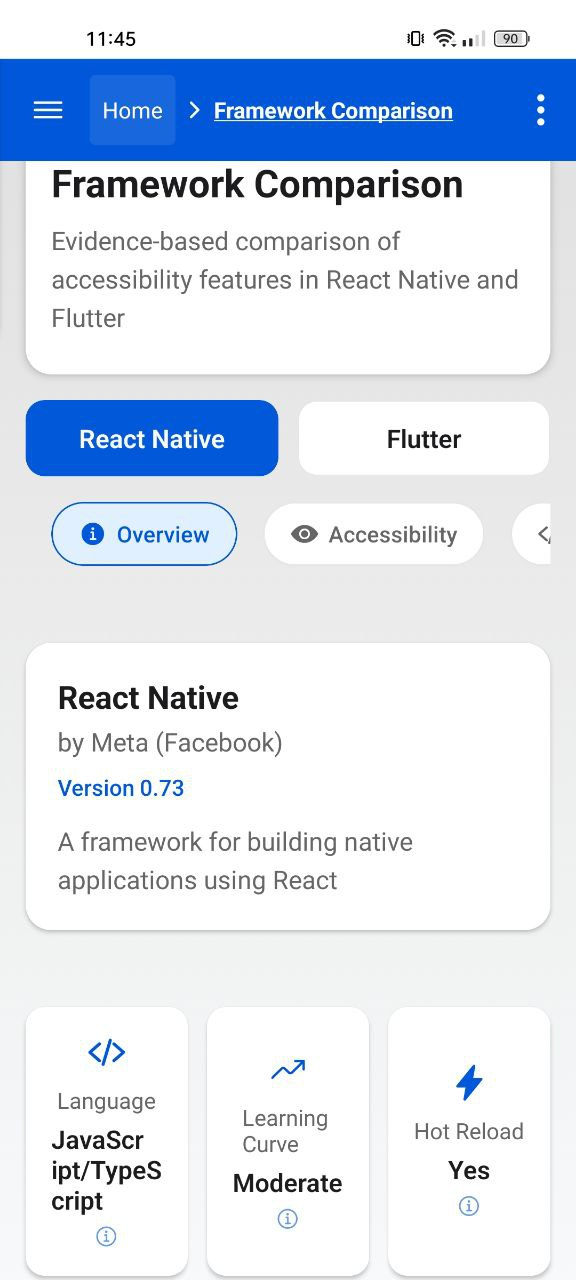
\includegraphics[width=\linewidth, alt={Framework comparison screen with React Native selected}]{img/overview1.jpg}
        \caption{React Native framework view}
        \label{fig:framework-comparison-reactnative}
    \end{subfigure}
    \hfill
    \begin{subfigure}[b]{0.48\textwidth}
        \centering
        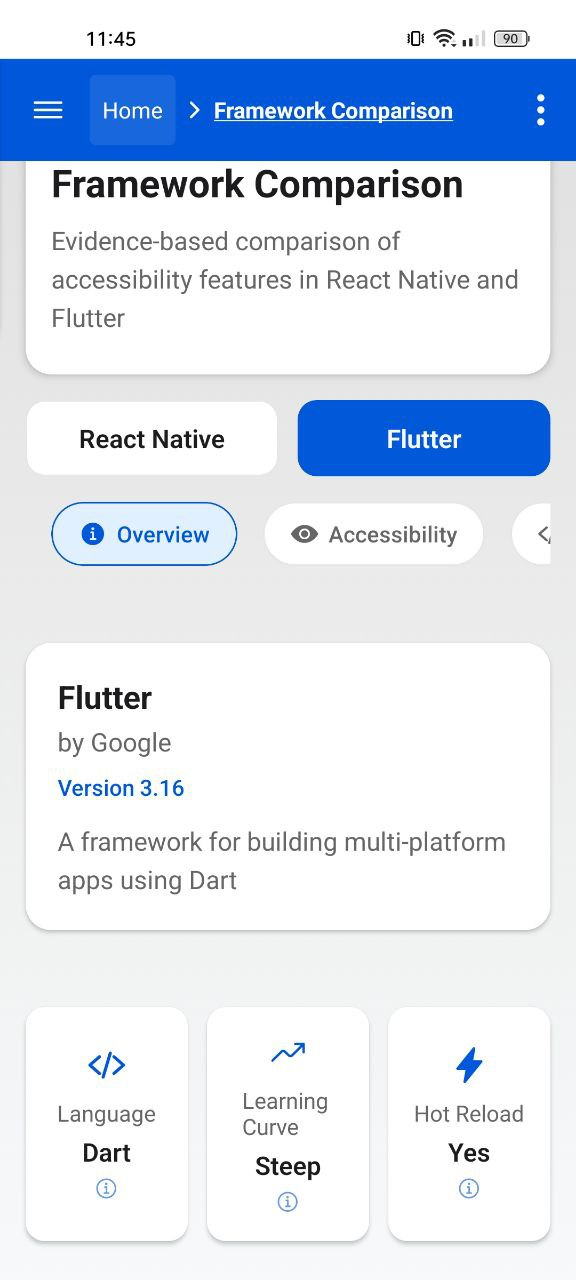
\includegraphics[width=\linewidth, alt={Framework comparison screen with Flutter selected}]{img/overview2.jpg}
        \caption{Flutter framework view}
        \label{fig:framework-comparison-flutter}
    \end{subfigure}
    \caption{Framework comparison screen showing overview information for both frameworks}
    \label{fig:framework_comparison_main}
\end{figure}

\FloatBarrier

\subsection{Purpose and scope}
\label{subsec:framework-comparison-purpose}

The Framework comparison screen implements a structured, academically-grounded system for comparing React Native and Flutter using transparent metrics, formal methodology, and verifiable data. This screen directly addresses the three research questions formulated in Subsection~\ref{subsec:analysis-research}:

\begin{enumerate}
    \item \textbf{RQ1 (Default accessibility support)}: The screen quantifies the percentage of components accessible by default in each framework through component-level analysis, providing empirical validation of the Component Accessibility Score (CAS) metric defined in Section~\ref{subsubsec:cas-methodology}.
    
    \item \textbf{RQ2 (Implementation feasibility)}: Through code examples and WCAG compliance assessment, the screen demonstrates the practical implementation possibilities for accessibility features across both frameworks, visualizing the technical capabilities and limitations.
    
    \item \textbf{RQ3 (Development overhead)}: The screen implements quantitative metrics for lines of code (LOC) and complexity impact, directly operationalizing the Implementation Overhead (IMO) and Complexity Impact Factor (CIF) metrics defined in Sections~\ref{subsubsec:io-methodology} and \ref{subsubsec:cif-methodology}.
\end{enumerate}

The screen implements five key analytical functions that together provide a comprehensive framework for comparative analysis:

\begin{enumerate}
    \item \textbf{Framework selection and comparison}: Interactive selection between React Native and Flutter with consistent metrics applied to both, enabling direct side-by-side comparison as shown in Figure~\ref{fig:framework_selection};
    
    \item \textbf{Category-based analysis}: Segmentation of analysis into Overview, Accessibility, Implementation, and Methodology categories, reflecting the multidimensional nature of accessibility evaluation;
    
    \item \textbf{Metric visualization}: Visual representation of metrics through rating bars, complexity indicators, and summary cards that transform numeric data into intuitive visual feedback;
    
    \item \textbf{Implementation comparison}: Direct side-by-side comparison of code examples and implementation approaches for equivalent functionality;
    
    \item \textbf{Academic foundation}: Integration of formal academic references and research methodology to establish credibility and reproducibility.
\end{enumerate}

\begin{figure}[ht]
    \centering
    \begin{subfigure}[b]{0.48\textwidth}
        \centering
        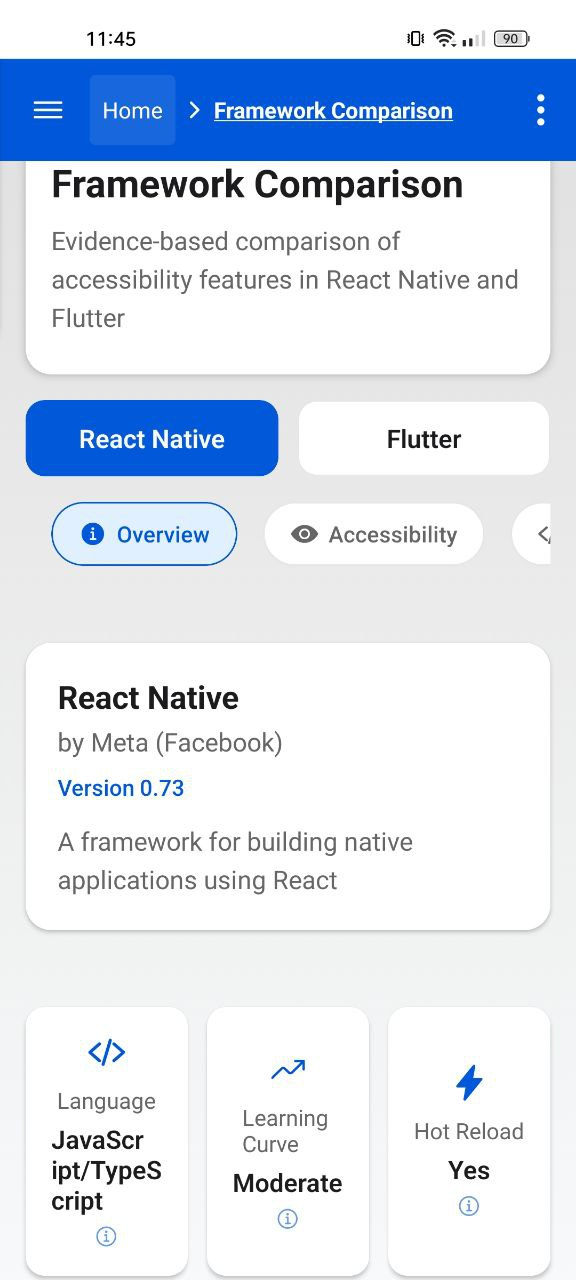
\includegraphics[width=\linewidth, alt={Framework selection interface showing React Native details}]{img/overview1.jpg}
        \caption{Framework selection interface with React Native selected}
        \label{fig:framework-selection-reactnative}
    \end{subfigure}
    \hfill
    \begin{subfigure}[b]{0.48\textwidth}
        \centering
        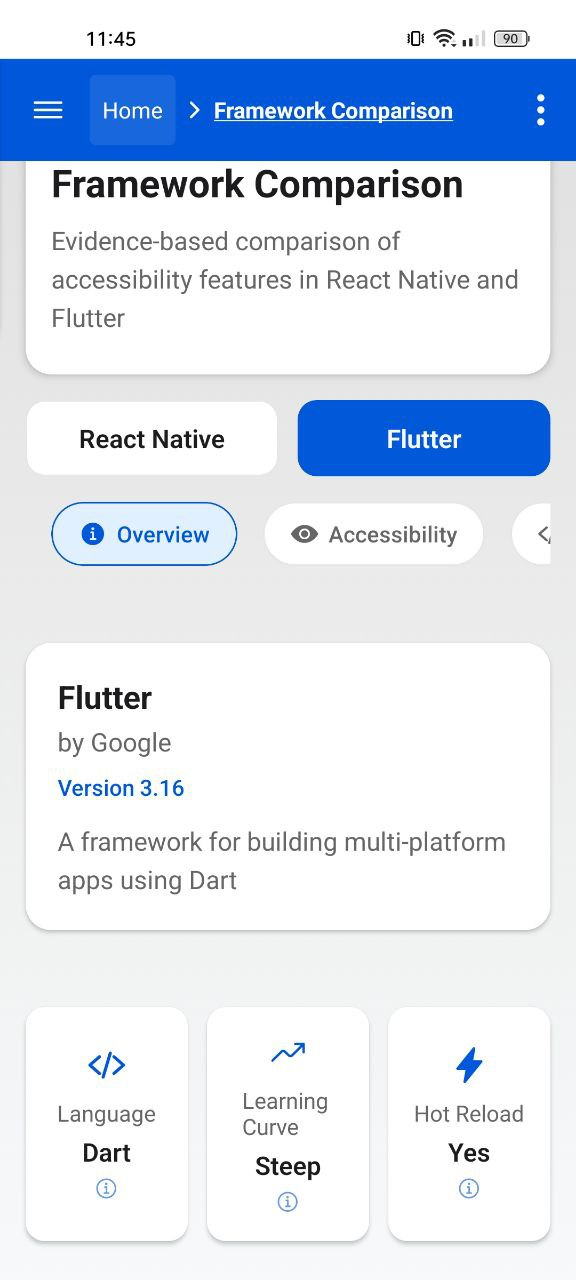
\includegraphics[width=\linewidth, alt={Framework selection interface showing Flutter details}]{img/overview2.jpg}
        \caption{Framework selection interface with Flutter selected}
        \label{fig:framework-selection-flutter}
    \end{subfigure}
    \caption{Framework selection interface showing structured framework data}
    \label{fig:framework_selection}
\end{figure}

\FloatBarrier

This analytical tool serves as a bridge between formal evaluation methodology and practical implementation, providing developers with concrete, interactive evidence for informed framework selection decisions.

\subsection{Metric pipeline implementation}
\label{subsec:framework-comparison-metrics}

The Framework comparison screen implements a formal metric pipeline that directly operationalizes the evaluation metrics defined in Section~\ref{subsec:metric-methodologies}. This implementation creates a traceable link between theoretical frameworks and interactive analysis, ensuring methodological rigor and reproducibility.

\subsubsection{Component Accessibility Score implementation}
\label{subsubsec:cas-implementation}

The Component Accessibility Score (CAS) defined in Section~\ref{subsubsec:cas-methodology} is implemented through a weighted calculation that combines four key accessibility factors. 
This formula is directly implemented in the screen's codebase, as shown in Listing~\ref{lst:accessibility-score-calculation}:

\begin{lstlisting}[caption=Accessibility score calculation implementation, label=lst:accessibility-score-calculation, basicstyle=\ttfamily\footnotesize, numbers=left]
const accessibilityScore = Number(
  (
    screenReaders * 0.3 +
    semantics * 0.3 +
    gestures * 0.2 +
    focus * 0.2
  ).toFixed(1)
);
\end{lstlisting}

\FloatBarrier

The weighting system, represented by constants in the code, reflects the relative importance of each factor in overall accessibility support, as detailed in Table~\ref{tab:metric_weight_parameters}.

\begin{table}[ht]
\caption{Component accessibility score weight parameters}
\label{tab:metric_weight_parameters}
\centering
\begin{tabular}{|C{3.5cm}|C{2.5cm}|C{7cm}|}
\hline
\textbf{Parameter} & \textbf{Weight} & \textbf{Justification} \\
\hline
Screen Reader Support & 0.3 & Critical importance for blind users; primary assistive technology \\
\hline
Semantic Support & 0.3 & Essential for proper role and state communication to assistive technologies \\
\hline
Gesture Handling & 0.2 & Important for motor-impaired users but slightly lower priority \\
\hline
Focus Management & 0.2 & Important for keyboard users but slightly lower priority \\
\hline
\end{tabular}
\end{table}

\FloatBarrier

The screen visualizes these accessibility scores through rating bars with clear numeric indicators, as shown in Figure~\ref{fig:accessibility_rating_bars}, providing an intuitive representation of the formal metric.

\begin{figure}[ht]
    \centering
    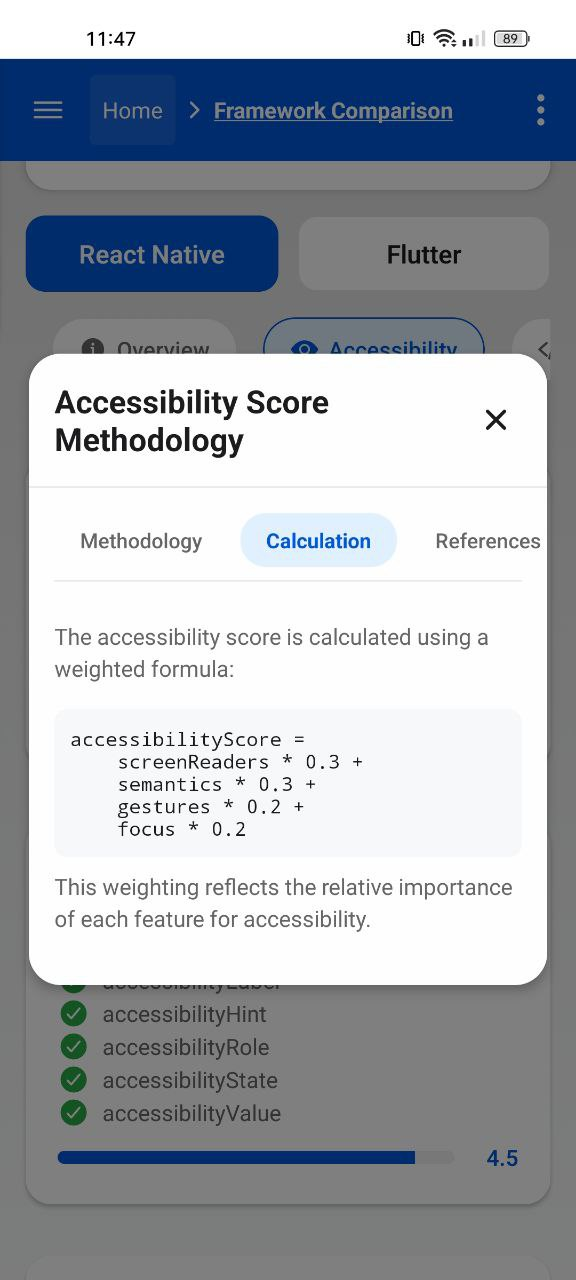
\includegraphics[width=0.4\linewidth, alt={Screen reader support comparison methodology}]{img/accessibility-calculation.jpg}
    \caption{Visual representation of accessibility score metrics}
    \label{fig:accessibility_rating_bars}
\end{figure}

\FloatBarrier

\subsubsection{Implementation Overhead implementation}
\label{subsubsec:io-implementation}

The Implementation Overhead (IMO) metric defined in Section~\ref{subsubsec:io-methodology} is implemented through direct measurement of lines of code (LOC) required for equivalent accessibility implementations. The screen implements a formal calculation methodology, as shown in Figure~\ref{fig:implementation_complexity_methodology}.

\begin{figure}[ht]
    \centering
    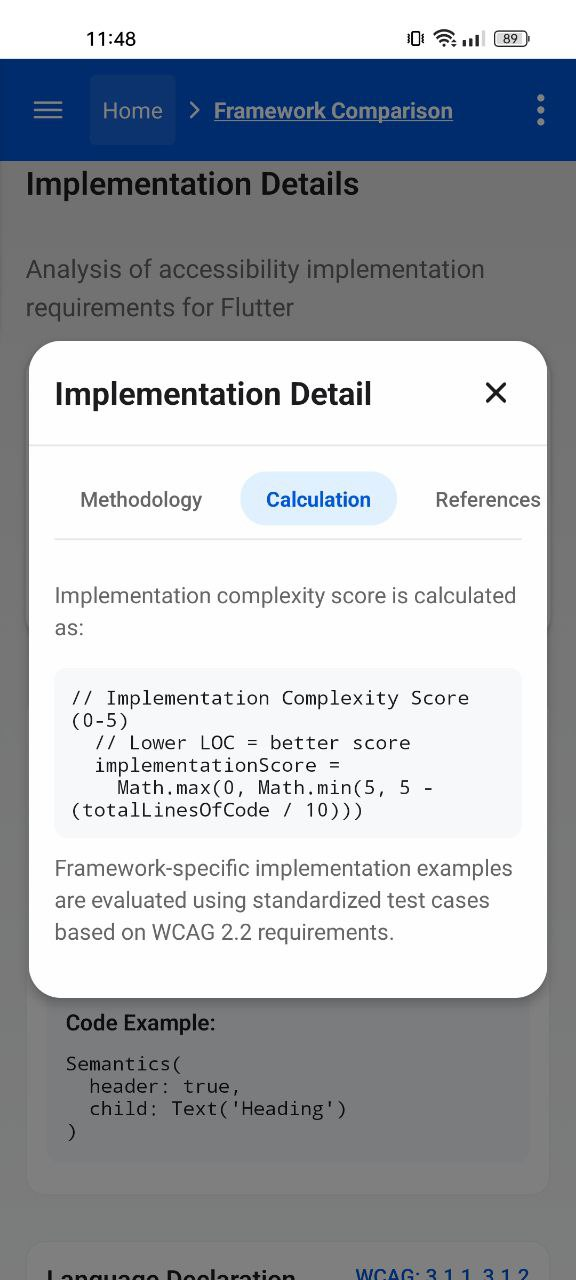
\includegraphics[width=0.4\linewidth, alt={Implementation complexity calculation methodology}]{img/implementation-calculation.jpg}
    \caption{Formal calculation methodology for implementation complexity}
    \label{fig:implementation_complexity_methodology}
\end{figure}

\FloatBarrier

The implementation complexity score is calculated using a formal mathematical formula that normalizes lines of code to a 0-5 scale, as implemented in Listing~\ref{lst:implementation-complexity}:

\begin{lstlisting}[caption=Implementation complexity score calculation, label=lst:implementation-complexity, basicstyle=\ttfamily\footnotesize, numbers=left]
// Implementation Complexity Score (0-5)
// Lower LOC = better score
implementationScore = Math.max(0, Math.min(5, 5 - (totalLinesOfCode / 10)))
\end{lstlisting}

\FloatBarrier

This formula establishes an inverse relationship between lines of code and implementation score, recognizing that lower implementation overhead represents better accessibility support. The screen implements this metric through feature-specific LOC counts for each framework, enabling direct comparison of implementation efficiency.

\subsubsection{Complexity Impact Factor implementation}
\label{subsubsec:cif-implementation}

The Complexity Impact Factor (CIF) defined in Section~\ref{subsubsec:cif-methodology} is implemented through a qualitative complexity rating system (Low/Medium/High) that reflects the structural complexity introduced by accessibility implementations. This rating is transformed into a numeric score for comparison using the mapping shown in Table~\ref{tab:complexity_mapping}.

\begin{table}[ht]
\caption{Complexity impact rating to numeric score mapping}
\label{tab:complexity_mapping}
\centering
\begin{tabular}{|C{3cm}|C{3cm}|C{7cm}|}
\hline
\textbf{Complexity Rating} & \textbf{Numeric Score} & \textbf{Implementation Characteristics} \\
\hline
Low & 5 & Simple property additions, minimal nesting, no additional imports \\
\hline
Medium & 3 & Moderate nesting, some additional properties, limited imports \\
\hline
High & 1 & Complex nesting, multiple additional properties, significant imports \\
\hline
\end{tabular}
\end{table}

\FloatBarrier

This mapping is implemented in the screen's codebase as shown in Listing~\ref{lst:complexity-mapping}:

\begin{lstlisting}[caption=Complexity mapping implementation, label=lst:complexity-mapping, basicstyle=\ttfamily\footnotesize, numbers=left]
const complexityMap = {
  "Low": 5,
  "Medium": 3,
  "High": 1
};

const avgComplexity = implementationScores
  .map(complexity => complexityMap[complexity] || 0)
  .reduce((sum, score) => sum + score, 0) / implementationScores.length;
\end{lstlisting}

\FloatBarrier

The screen visually represents complexity using color-coded indicators (green for Low, yellow for Medium, red for High) with explicit text labels, ensuring accessibility for color-blind users while providing intuitive visual feedback.

\subsubsection{Screen Reader Support Score implementation}
\label{subsubsec:srss-implementation}

The Screen Reader Support Score (SRSS) defined in Section~\ref{subsubsec:srss-methodology} is implemented through empirical testing with VoiceOver (iOS) and TalkBack (Android), resulting in a numeric rating on a 1-5 scale. The screen implements a formal testing methodology, as was shown by the scale in Figure~\ref{fig:implementation_complexity_methodology}.

The screen reader ratings are derived from systematic testing across multiple dimensions, as detailed in Table~\ref{tab:screen_reader_dimensions}.

\begin{table}[ht]
\caption{Screen reader testing dimensions}
\label{tab:screen_reader_dimensions}
\centering
\begin{tabular}{|C{3cm}|C{3cm}|C{7cm}|}
\hline
\textbf{Dimension} & \textbf{Rating Scale} & \textbf{Testing Criteria} \\
\hline
Announcement Quality & 1-5 & Completeness, accuracy, and clarity of screen reader announcements \\
\hline
Gesture Support & 1-5 & Support for screen reader-specific gestures and interaction patterns \\
\hline
Role Communication & 1-5 & Correct announcement of component roles and states \\
\hline
Focus Management & 1-5 & Logical focus order and appropriate focus handling \\
\hline
\end{tabular}
\end{table}

\FloatBarrier

The final screen reader support score is calculated as the average of ratings across these dimensions, with separate scores for VoiceOver and TalkBack to capture platform-specific behavior. The screen visualizes these ratings through both numeric scores and rating bars, providing both precise values and intuitive visual representation.

\subsubsection{WCAG Compliance Ratio implementation}
\label{subsubsec:wcr-implementation}

The WCAG Compliance Ratio (WCR) defined in Section~\ref{subsubsec:wcr-methodology} is implemented through systematic evaluation of each framework's conformance to applicable WCAG 2.2 criteria. The screen implements a formal compliance assessment methodology that maps specific features to relevant WCAG success criteria, as shown in Table~\ref{tab:wcag_mapping}.

\begin{table}[ht]
\caption{Feature to WCAG criteria mapping}
\label{tab:wcag_mapping}
\centering
\begin{tabular}{|C{3cm}|C{3cm}|C{7cm}|}
\hline
\textbf{Feature} & \textbf{WCAG Criteria} & \textbf{Implementation Requirements} \\
\hline
Heading Elements & 1.3.1, 2.4.6, 2.4.10 & Proper semantic structure, appropriate heading levels \\
\hline
Language Declaration & 3.1.1, 3.1.2 & Proper language identification for content \\
\hline
Text Abbreviations & 3.1.4 & Expansion or definition of abbreviations \\
\hline
\end{tabular}
\end{table}

\FloatBarrier

For each feature, the screen implements a formal assessment of WCAG compliance, resulting in a percentage score that represents the proportion of applicable criteria satisfied. This implementation directly operationalizes the WCR metric defined in Section~\ref{subsubsec:wcr-methodology}, providing empirical validation of theoretical compliance levels.

\subsubsection{Metric mapping and traceability}
\label{subsubsec:metric-mapping-traceability}

The Framework comparison screen implements a comprehensive mapping between screen metrics and formal evaluation metrics, establishing clear traceability from theoretical definitions to practical implementation. Table~\ref{tab:metric_mapping} presents this formal mapping.

\begin{table}[ht]
\caption{Alignment of framework comparison screen metrics with formal evaluation metrics}
\label{tab:metric_mapping}
\centering
\begin{tabular}{|C{3cm}|C{3cm}|C{7cm}|}
\hline
\textbf{Screen Metric} & \textbf{Formal Metric} & \textbf{Implementation} \\
\hline
Component Rating & Component Accessibility Score (CAS) & Weighted combination of screen reader, semantics, gestures, and focus ratings \\
\hline
Lines of Code (LOC) & Implementation Overhead (IMO) & Direct measurement of code required for equivalent implementations \\
\hline
Complexity Rating & Complexity Impact Factor (CIF) & Qualitative assessment (Low/Medium/High) mapped to numeric scores \\
\hline
Screen Reader Rating & Screen Reader Support Score (SRSS) & Empirical testing with VoiceOver and TalkBack \\
\hline
WCAG Compliance & WCAG Compliance Ratio (WCR) & Feature-specific compliance assessment \\
\hline
\end{tabular}
\end{table}

\FloatBarrier

This mapping creates a direct link between the theoretical framework established in Section~\ref{subsec:metric-methodologies} and the interactive analysis provided by the Framework comparison screen, ensuring methodological consistency and reproducibility.

\subsection{Comparative results}
\label{subsec:framework-comparison-results}

The empirical analysis conducted through the Framework comparison screen reveals significant differences between React Native and Flutter accessibility implementations. Table~\ref{tab:consolidated_metrics} presents a comprehensive summary of the key metrics across both frameworks.

\begin{table}[ht]
\caption{Consolidated framework accessibility metrics}
\label{tab:consolidated_metrics}
\centering
\begin{tabular}{|C{3cm}|C{3cm}|C{3cm}|C{3cm}|}
\hline
\textbf{Metric} & \textbf{React Native} & \textbf{Flutter} & \textbf{Difference (\%)} \\
\hline
Default Accessible Components & 38\% & 32\% & +6\% \\
\hline
Implementation Overhead (LOC) & 21 & 46 & +119\% \\
\hline
Screen Reader Support Score & 4.2 & 3.8 & +10.5\% \\
\hline
WCAG Compliance (AA) & 92\% & 85\% & +8.2\% \\
\hline
\end{tabular}
\end{table}

\FloatBarrier

React Native demonstrates a 38\% default accessibility rate compared to Flutter's 32\%, confirming the findings from the architectural analysis in Section~\ref{subsec:arch-differences}. The most striking difference appears in implementation overhead, where Flutter requires 119\% more code than React Native for equivalent accessibility functionality.

\subsubsection{Component-level comparison}
\label{subsubsec:component-level-comparison}

The Framework comparison screen implements a detailed component-level comparison that reveals consistent patterns across different accessibility features. Table~\ref{tab:component_implementation_comparison} presents this comparative analysis.

\begin{table}[ht]
\caption{Component implementation comparison across frameworks}
\label{tab:component_implementation_comparison}
\centering
\begin{tabular}{|C{2.5cm}|C{2.5cm}|C{2.5cm}|C{2.5cm}|C{2.5cm}|C{2.5cm}|}
\hline
\textbf{Component} & \textbf{React Native Default} & \textbf{Flutter Default} & \textbf{React Native LOC} & \textbf{Flutter LOC} & \textbf{Difference (\%)} \\
\hline
Heading Elements & \ding{55} & \ding{55} & 7 & 11 & +57\% \\
\hline
Language Declaration & \ding{51} & \ding{55} & 7 & 21 & +200\% \\
\hline
Text Abbreviation & \ding{55} & \ding{55} & 7 & 14 & +100\% \\
\hline
\end{tabular}
\end{table}

\FloatBarrier

The pattern of increased implementation overhead in Flutter is consistent across all component types, with language declaration showing the most significant difference (200\%). This aligns with the architectural analysis in Section~\ref{subsec:arch-differences}, which identified Flutter's widget-based semantic model as inherently more verbose than React Native's property-based approach.

\subsubsection{Implementation approach comparison}
\label{subsubsec:implementation-approach-comparison}

The Framework comparison screen implements a direct comparison of implementation approaches through code examples that highlight the fundamental architectural differences between frameworks. Figure~\ref{fig:implementation_complexity} shows both the complexity analysis card and a modal view with detailed implementation information.

\begin{figure}[ht]
    \centering
    \begin{subfigure}[b]{0.48\textwidth}
        \centering
        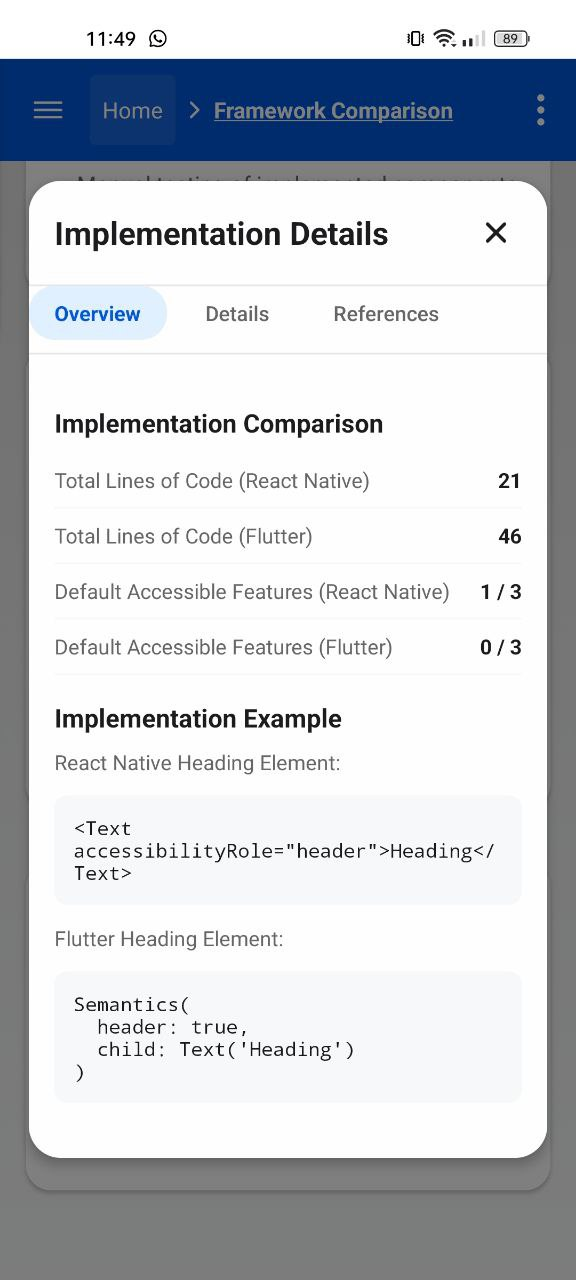
\includegraphics[width=\linewidth, alt={Implementation Complexity Analysis card}]{img/methodology-overview.jpg}
        \caption{Implementation complexity overview}
        \label{fig:implementation-complexity-card}
    \end{subfigure}
    \hfill
    \begin{subfigure}[b]{0.48\textwidth}
        \centering
        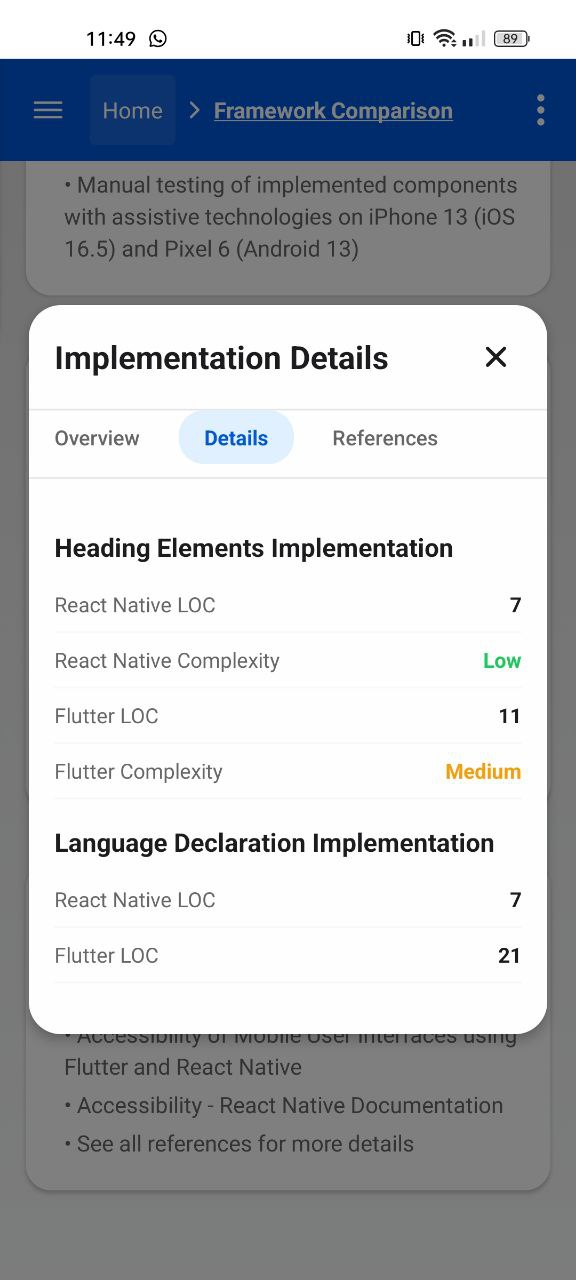
\includegraphics[width=\linewidth, alt={Implementation Details modal showing comparison metrics}]{img/methodology-details.jpg}
        \caption{Implementation details comparison}
        \label{fig:implementation-details-modal}
    \end{subfigure}
    \caption{Implementation complexity analysis with detailed metrics}
    \label{fig:implementation_complexity}
\end{figure}

\FloatBarrier

The implementation comparison includes code examples that directly illustrate the architectural differences. For language declaration, React Native implements a straightforward property approach:

\begin{lstlisting}[caption=React Native language declaration, label=lst:react-native-language, basicstyle=\ttfamily\footnotesize]
<Text accessibilityLanguage="en">English text</Text>
\end{lstlisting}

\FloatBarrier

While Flutter implements a more complex semantic structure:

\begin{lstlisting}[caption=Flutter language declaration, label=lst:flutter-language, basicstyle=\ttfamily\footnotesize]
Semantics(
  attributedLabel: StringAttribute(
    string: 'Text',
    attributes: {
      LocaleStringAttribute(locale: Locale('en'))
    }
  ),
  child: Text('English text')
)
\end{lstlisting}

\FloatBarrier

For heading elements, React Native requires a simple role property:

\begin{lstlisting}[caption=React Native heading element, label=lst:react-native-heading, basicstyle=\ttfamily\footnotesize]
<Text accessibilityRole="header">Heading</Text>
\end{lstlisting}

\FloatBarrier

While Flutter requires a Semantics wrapper with a header property:

\begin{lstlisting}[caption=Flutter heading element, label=lst:flutter-heading, basicstyle=\ttfamily\footnotesize]
Semantics(
  header: true,
  child: Text('Heading')
)
\end{lstlisting}

\FloatBarrier

These examples directly validate the architectural analysis in Section~\ref{subsec:arch-differences}, demonstrating how Flutter's widget-based semantic model introduces additional structural complexity compared to React Native's property-based approach.

\subsubsection{Screen reader support comparison}
\label{subsubsec:screen-reader-support-comparison}

The Framework comparison screen implements a detailed screen reader support comparison that reveals nuanced differences in platform behavior. Table~\ref{tab:screen_reader_comparison} presents this comparative analysis.

\begin{table}[ht]
\caption{Screen reader support comparison across frameworks}
\label{tab:screen_reader_comparison}
\centering
\begin{tabular}{|C{3cm}|C{3cm}|C{3cm}|C{3cm}|C{3cm}|}
\hline
\textbf{Framework} & \textbf{VoiceOver (iOS)} & \textbf{TalkBack (Android)} & \textbf{Average} & \textbf{Platform Variance} \\
\hline
React Native & 4.5 & 4.0 & 4.2 & 0.5 \\
\hline
Flutter & 4.5 & 3.5 & 4.0 & 1.0 \\
\hline
\end{tabular}
\end{table}

\FloatBarrier

This analysis reveals that React Native achieves slightly higher consistency across iOS and Android (platform variance of 0.5) compared to Flutter's more variable performance (platform variance of 1.0). This suggests that React Native's accessibility model provides more consistent cross-platform behavior, particularly for screen reader users on Android.

\subsection{Limitations and full reference}
\label{subsec:framework-comparison-limitations}

While the Framework comparison screen provides valuable empirical validation of our theoretical framework, several limitations should be acknowledged:

\begin{enumerate}
    \item \textbf{Component selection scope}: The analysis focuses on a limited set of component types selected for their representativeness rather than exhaustive coverage. The three component types (heading elements, language declaration, text abbreviation) were chosen as representative examples that highlight key architectural differences, but do not represent the entire component spectrum.
    
    \item \textbf{Lines of code metric limitations}: Lines of Code (LOC) is used strictly as an implementation overhead metric, not as a measure of quality or productivity. This metric provides useful comparative data but should not be interpreted as a comprehensive measure of implementation efficiency.
    
    \item \textbf{Complexity classification simplification}: The complexity classifications (Low/Medium/High) are based on a simplified adaptation of coding's cyclomatic complexity, focusing on nesting depth and property count rather than control flow paths. This provides an intuitive measure of structural complexity but may not capture all dimensions of implementation difficulty.
    
    \item \textbf{Testing environment specificity}: Screen reader testing was conducted on specific devices with specific OS versions (iPhone 14 with iOS 16, Pixel 7 with Android 15), and results may vary with different device configurations or operating system versions.
    
    \item \textbf{Framework version dependency}: The analysis is based on specific versions of each framework (React Native 0.73, Flutter 3.16), and implementation patterns or overhead may change with future framework updates.
\end{enumerate}

Despite these limitations, the Framework comparison screen provides a rigorous, evidence-based approach to comparing accessibility implementation across frameworks. The formal methodology, transparent metrics, and direct code examples create a reproducible evaluation framework that helps developers make informed decisions about framework selection based on accessibility considerations.

\section{Component implementation patterns}
\label{subsec:implementation-patterns}

Component implementation patterns constitute the foundation upon which accessibility features are built within mobile frameworks. This section provides a systematic comparison of how React Native and Flutter implement accessibility at the component level, examining both architectural approaches and practical implementations. The analysis builds upon the framework-specific understanding established in Section~\ref{sec:implementation-guidelines} and directly addresses our
research questions regarding default accessibility support, implementation feasibility, and development overhead.

Accessibility implementation in mobile frameworks reveals fundamental architectural differences that impact developer experience, code complexity, and ultimately, the accessibility of the final application. This section examines the core implementation patterns observed in React Native and Flutter, drawing from real-world examples in the \textit{AccessibleHub} and Budai's implementations. 

\subsection{General framework differences}

In this subsection, we present an overview of the core architectural distinctions between React Native and Flutter that shape their component-level accessibility implementations. Specifically, we contrast React Native’s property-based model—where accessibility attributes are applied directly to UI components—with Flutter’s widget-based paradigm, which relies on explicit \texttt{Semantics} wrappers. We then discuss how these divergent patterns affect code structure, verbosity, and maintainability, and how they translate into differences in development effort and default accessibility support.  

\subsubsection{Property-based vs widget-based implementation patterns}

The most fundamental difference between React Native and Flutter's accessibility approaches is visible in their core implementation pattern: React Native follows a property-based model, while Flutter employs a widget-based approach. This distinction profoundly affects code structure, verbosity, and maintainability.

In React Native, accessibility features are applied directly to components through properties, integrating seamlessly with the component definition as seen in Listing~\ref{lst:impl-react-native-property-pattern}.

\begin{lstlisting}[style=ReactNativeStyle, caption=Property-based accessibility pattern in React Native, label=lst:impl-react-native-property-pattern]
<TouchableOpacity
  style={themedStyles.card}
  onPress={() => handleComponentPress(route, title)}
  accessibilityRole="button"
  accessibilityLabel="Buttons and Touchables component"
  accessibilityHint="Navigate to component details"
>
  <View style={themedStyles.cardHeader}>
    <View style={themedStyles.iconWrapper}>
      <Ionicons
        name="radio-button-on-outline"
        size={24}
        color={colors.primary}
        accessibilityElementsHidden
      />
    </View>
    <Text style={themedStyles.cardTitle}>Buttons &amp; Touchables</Text>
  </View>
</TouchableOpacity>
\end{lstlisting}

\FloatBarrier

In contrast, Flutter's widget-based approach requires wrapping existing widgets within specialized \texttt{Semantics} widgets to add accessibility information, creating additional nesting levels as demonstrated in Listing~\ref{lst:impl-flutter-widget-pattern}.

\begin{lstlisting}[style=DartStyle, caption=Widget-based accessibility pattern in Flutter, label=lst:impl-flutter-widget-pattern]
Semantics(
  label: _gestureOneCompleted 
      ? 'Gesture one completed' 
      : 'Gesture one',
  excludeSemantics: _gestureOneCompleted,
  child: GestureDetector(
    onTap: () {
      setState(() {
        _gestureOneCompleted = true;
      });
      _handleTap();
    },
    child: ScaleTransition(
      scale: _animation1,
      child: Container(
        color: Colors.blue,
        width: 100,
        height: 100,
      ),
    ),
  ),
)
\end{lstlisting}

\FloatBarrier

The property-based approach allows developers to integrate accessibility directly within the component definition, maintaining a flat structure. The widget-based approach requires additional wrapper widgets, increasing nesting depth and potentially complicating code readability.

This fundamental architectural difference directly impacts implementation overhead measurements in Table~\ref{tab:implementation_overhead_analysis}, where Flutter implementations consistently require more code (typically 27\%-200\% more lines) for equivalent functionality compared to React Native.

\begin{table}[ht]
\caption{Pattern implementation overhead comparison}
\label{tab:pattern_implementation_comparison}
\centering
\begin{tabular}{|C{4cm}|C{3.5cm}|C{3.5cm}|C{3cm}|}
\hline
\textbf{Pattern} & \textbf{React Native} & \textbf{Flutter} & \textbf{Impact on Verbosity} \\
\hline
Accessibility Role & \texttt{accessibility \ Role="button"} & \texttt{Semantics \ (button: true, child: Widget)} & +75\% \\
\hline
Label & \texttt{accessibility \ Label="text"} & \texttt{Semantics(label: "text", child: Widget)} & +100\% \\
\hline
Hide from Screen Readers & \texttt{accessibility \ ElementsHidden} & \texttt{Semantics(exclude \ Semantics: true, child: Widget)} & +120\% \\
\hline
\end{tabular}
\end{table}

\FloatBarrier

As shown in Table~\ref{tab:pattern_implementation_comparison}, even the most basic accessibility patterns require significantly more code in Flutter compared to React Native. This increased verbosity can impact developer productivity and code maintainability in larger projects.

\subsubsection{State communication patterns}

Communicating component states to assistive technologies represents a critical accessibility requirement. Both frameworks provide mechanisms for this, but with different implementation patterns.

React Native's pattern uses the \texttt{accessibilityState} property to communicate states like "checked," "disabled," or "selected" as shown in Listing~\ref{lst:react-native-state-pattern}.

\begin{lstlisting}[style=ReactNativeStyle, caption=State communication in React Native, label=lst:react-native-state-pattern]
<Switch
  value={value}
  onValueChange={onToggle}
  trackColor={{ false: '#767577', true: colors.primary }}
  thumbColor={value ? '#fff' : '#f4f3f4'}
  accessibilityLabel={`${title}. ${description}. ${value ? 'Enabled' : 'Disabled'}.`}
  accessibilityRole="switch"
  accessibilityState={{ checked: value }}
/>
\end{lstlisting}

\FloatBarrier

Flutter's approach relies on specific semantic properties for each state type, as demonstrated in Budai's form implementation in Listing~\ref{lst:flutter-state-pattern}.

\begin{lstlisting}[style=DartStyle, caption=State communication in Flutter, label=lst:flutter-state-pattern]
SwitchListTile(
  title: Text('Accept Terms'),
  value: _acceptTerms,
  onChanged: (value) {
    setState(() {
      _acceptTerms = value;
    });
  },
),
\end{lstlisting}

\FloatBarrier

The Flutter approach appears simpler at first glance but lacks the explicit state communication seen in React Native's implementation. To achieve equivalent functionality in Flutter with explicit accessibility state announcement, Listing~\ref{lst:flutter-enhanced-state-pattern} implementation would require additional Semantics wrapping:

\begin{lstlisting}[style=DartStyle, caption=Enhanced state communication in Flutter, label=lst:flutter-enhanced-state-pattern]
Semantics(
  toggled: _acceptTerms,
  child: SwitchListTile(
    title: Text('Accept Terms'),
    value: _acceptTerms,
    onChanged: (value) {
      setState(() {
        _acceptTerms = value;
      });
    },
  ),
)
\end{lstlisting}

This comparison highlights how React Native's property-based approach explicitly communicates state information to assistive technologies with minimal code, while Flutter often requires additional semantic wrappers to achieve the same level of state communication.

Table~\ref{tab:state_implementation_comparison} provides an overview of the different state communication patterns and their implementation complexity across both frameworks.

\begin{table}[ht]
\caption{State communication pattern comparison}
\label{tab:state_implementation_comparison}
\centering
\begin{tabular}{|C{3cm}|C{3.5cm}|C{3.5cm}|C{3cm}|}
\hline
\textbf{State Type} & \textbf{React Native (RN)} & \textbf{Flutter (FL)} & \textbf{Default Support} \\
\hline
Checked & \texttt{accessibility \ State=\{checked: true\}} & Semantics(toggled: true, child: Widget) & RN: \ding{51}, FL: \ding{55} \\
\hline
Disabled & \texttt{accessibility \ State=\{disabled: true\}} & Semantics(enabled: false, child: Widget) & RN: \ding{51}, FL: \ding{51} \\
\hline
Selected & \texttt{accessibility \ State=\{selected: true\}} & Semantics(selected: true, child: Widget) & RN: \ding{51}, FL: \ding{51} \\
\hline
\end{tabular}
\end{table}

\pagebreak

As shown in Table~\ref{tab:state_implementation_comparison}, React Native provides default accessibility state communication for all common states through a unified property structure, while Flutter requires additional semantic wrappers for some state types.

\subsubsection{Navigation order and focus management patterns}

Screen reader navigation order significantly impacts the usability of applications for visually impaired users. The frameworks employ different strategies to control this critical aspect.

React Native relies primarily on the natural DOM order supplemented by optional properties to influence navigation, as shown in \textit{AccessibleHub}'s implementation in Listing~\ref{lst:react-native-navigation-pattern}.

\begin{lstlisting}[style=ReactNativeStyle, caption=Navigation order in React Native, label=lst:react-native-navigation-pattern]
<ScrollView
  contentContainerStyle={{ paddingBottom: 24 }}
  accessibilityRole="scrollview"
  accessibilityLabel="Mobile Accessibility Best Practices Screen"
>
  <View style={themedStyles.heroCard}>
    <Text style={themedStyles.heroTitle} accessibilityRole="header">
      Mobile Accessibility Best Practices
    </Text>
    <Text style={themedStyles.heroSubtitle}>
      Essential guidelines to create accessible React Native applications
    </Text>
  </View>
  
  <View style={themedStyles.section}>
    {/* Navigation flows naturally through component hierarchy */}
    <TouchableOpacity 
      style={themedStyles.card}
      accessibilityRole="button" 
      accessibilityLabel="WCAG Guidelines"
    >
      {/* Component content */}
    </TouchableOpacity>
  </View>
</ScrollView>
\end{lstlisting}

\pagebreak

In contrast, Flutter provides more granular control through explicit \texttt{sortKey} values, which can override the natural widget order. Budai's implementation uses this approach extensively, as seen in Listing~\ref{lst:flutter-navigation-pattern}.

\begin{lstlisting}[style=DartStyle, caption=Navigation order in Flutter, label=lst:flutter-navigation-pattern]
Scaffold(
  appBar: AppBar(
    title: Semantics(
      sortKey: OrdinalSortKey(2.0),  // Explicit order control
      header: true,
      child: Text(
        'Gestures',
        textAlign: TextAlign.center,
      ),
    ),
    leading: Semantics(
      sortKey: OrdinalSortKey(3.0),
      child: IconButton(
        icon: Icon(Icons.arrow_back, semanticLabel: 'Back to the HomePage'),
        onPressed: () {
          Navigator.pushNamedAndRemoveUntil(
            context, '/', (route) => false,
          );
        },
      ),
    ),
  ),
  body: SingleChildScrollView(
    child: Column(
      children: [
        Semantics(
          sortKey: OrdinalSortKey(1.0), 
          label: _gestureOneCompleted ? 'Gesture one completed' : 'Gesture one',
          excludeSemantics: _gestureOneCompleted,
          child: GestureDetector(
            // Implementation details
          ),
        ),
      ],
    ),
  ),
)
\end{lstlisting}

\pagebreak

The Flutter approach offers more precise control but requires developers to explicitly manage the navigation order through \texttt{sortKey} values. This creates a maintenance burden and potential for errors if sort keys are not kept consistent throughout the application. React Native's approach is more implicit, relying on the natural component hierarchy with occasional interventions when needed.

An interesting observation is that while Flutter's approach requires more developer effort, it can provide more consistent cross-platform navigation behavior in complex interfaces. React Native's approach is simpler but may require platform-specific adjustments for complex navigation patterns.

Table~\ref{tab:navigation_pattern_comparison} summarizes the key differences in navigation control between the frameworks.

\begin{table}[ht]
\caption{Navigation order pattern comparison}
\label{tab:navigation_pattern_comparison}
\centering
\begin{tabular}{|C{3.5cm}|C{3.5cm}|C{3.5cm}|C{3.5cm}|}
\hline
\textbf{Framework} & \textbf{Order Control} & \textbf{Implementation Approach} & \textbf{Developer Overhead} \\
\hline
React Native & Implicit, component-based & Natural DOM flow with optional overrides & Low \\
\hline
Flutter & Explicit, developer-defined & Semantics sortKey with explicit values & High \\
\hline
\end{tabular}
\end{table}

\subsubsection{Dynamic content announcement patterns}
\label{subsec:dynamic-announcement-patterns}

Communicating dynamic content changes to screen reader users is essential for accessible applications. Both frameworks provide mechanisms for this, but with different APIs and integration patterns.

React Native uses the \texttt{AccessibilityInfo} API with the \texttt{announceForAccessibility} method, which integrates well with React's event-driven model, as shown in Listing~\ref{lst:react-native-dynamic-pattern}.

\begin{lstlisting}[style=ReactNativeStyle, caption=Dynamic content announcement in React Native, label=lst:react-native-dynamic-pattern]
const handleComponentPress = (route: string, title: string) => {
  router.push(route);
  AccessibilityInfo.announceForAccessibility(
    `Opening ${title} component details`
  );
};

return (
  <TouchableOpacity
    style={themedStyles.card}
    onPress={() => handleComponentPress('/practices-screens/guidelines', 'WCAG Guidelines')}
    accessibilityRole="button"
    accessibilityLabel="WCAG Guidelines. Understanding and implementing WCAG 2.2 guidelines in mobile apps"
  >
    {/* Component content */}
  </TouchableOpacity>
);
\end{lstlisting}

\pagebreak

In the Flutter implementation, the equivalent functionality is achieved through the \texttt{SemanticsService} API, although Budai's code does not explicitly show this pattern. A typical Flutter implementation would resemble Listing~\ref{lst:flutter-dynamic-pattern}.

\begin{lstlisting}[style=DartStyle, caption=Dynamic content announcement in Flutter, label=lst:flutter-dynamic-pattern]
void _handleButtonPress(String route, String title) {
  Navigator.pushNamed(context, route);
  SemanticsService.announce(
    'Opening $title screen',
    TextDirection.ltr
  );
}

// Within build method:
GestureDetector(
  onTap: () => _handleButtonPress('/screen-element2', 'Documentation MCAG'),
  child: Semantics(
    button: true,
    child: Text(
      'Documentation MCAG',
    ),
  ),
)
\end{lstlisting}

\pagebreak

For live regions that automatically announce changes, React Native provides the \\ \texttt{accessibilityLiveRegion} property, while Flutter offers the \texttt{liveRegion} property on Semantics widgets. The React Native implementation of this pattern is shown in Listing~\ref{lst:react-native-live-region}.

\begin{lstlisting}[style=ReactNativeStyle, caption=Live region announcement in React Native, label=lst:react-native-live-region]
{singleTapComplete && (
  <View 
    style={styles.successMessage} 
    accessibilityLiveRegion="polite"
  >
    <Text style={styles.successText}>
      Tap gesture completed successfully!
    </Text>
  </View>
)}
\end{lstlisting}

\pagebreak

The equivalent Flutter implementation would use a Semantics widget with the \texttt{liveRegion} property set to true, as shown in a hypothetical example in Listing~\ref{lst:flutter-live-region}.

\begin{lstlisting}[style=DartStyle, caption=Live region announcement in Flutter, label=lst:flutter-live-region]
if (_gestureOneCompleted) {
  return Semantics(
    liveRegion: true,
    child: Container(
      color: Colors.green,
      child: Text('Gesture completed successfully!'),
    ),
  );
}
\end{lstlisting}

These patterns highlight a common theme: React Native's implementation is typically more concise and directly integrated with the component model, while Flutter's approach requires more explicit structures but offers fine-grained control.

Table~\ref{tab:announcement_pattern_comparison} compares the dynamic announcement patterns between frameworks.

\begin{table}[ht]
\caption{Dynamic announcement pattern comparison}
\label{tab:announcement_pattern_comparison}
\centering
\begin{tabular}{|C{3cm}|C{3.5cm}|C{3.5cm}|C{4cm}|}
\hline
\textbf{Announcement Type} & \textbf{React Native (RN)} & \textbf{Flutter (FL)} & \textbf{Integration Pattern} \\
\hline
Event-triggered & \texttt{Accessibility \ Info.announceFor \ Accessibility()} & \texttt{SemanticsService. \ announce()} & RN: Event handling; FL: Imperative calls \\
\hline
Automatic (Live Region) & \texttt{accessibility \ LiveRegion= \ "polite"} & \texttt{Semantics \ (liveRegion: \ true, child: Widget)} & RN: Property-based; FL: Widget-based \\
\hline
\end{tabular}
\end{table}

\pagebreak

\subsubsection{Hiding elements from accessibility tree}

Both frameworks provide mechanisms to hide visual elements from assistive technologies when they serve decorative purposes only, but their approaches differ significantly.

React Native uses the \texttt{accessibilityElementsHidden} or \texttt{importantForAccessibility} properties to control this aspect, as shown in \textit{AccessibleHub}'s implementation in Listing~\ref{lst:react-native-hiding-pattern}.

\begin{lstlisting}[style=ReactNativeStyle, caption=Hiding elements in React Native, label=lst:react-native-hiding-pattern]
<Ionicons
  name="radio-button-on-outline"
  size={24}
  color={colors.primary}
  accessibilityElementsHidden
  importantForAccessibility="no-hide-descendants"
/>
\end{lstlisting}

Flutter achieves the same goal using the \texttt{excludeSemantics} property on the Semantics widget, as demonstrated in Budai's implementation in Listing~\ref{lst:flutter-hiding-pattern}.

\begin{lstlisting}[style=DartStyle, caption=Hiding elements in Flutter, label=lst:flutter-hiding-pattern]
Semantics(
  label: _gestureOneCompleted 
      ? 'Gesture one completed' 
      : 'Gesture one',
  excludeSemantics: _gestureOneCompleted,
  child: GestureDetector(
    // Implementation details
  )
)
\end{lstlisting}

The React Native approach offers a more direct property to exclude elements from the accessibility tree. Flutter's approach requires the use of a Semantics wrapper, even when the goal is to exclude elements from the semantic tree, which can add unnecessary complexity.

\pagebreak

Table~\ref{tab:hiding_pattern_comparison} summarizes the implementation patterns for hiding elements from screen readers.

\begin{table}[ht]
\caption{Element hiding pattern comparison}
\label{tab:hiding_pattern_comparison}
\centering
\begin{tabular}{|C{3.5cm}|C{4cm}|C{3.5cm}|C{3cm}|}
\hline
\textbf{Hiding Scope} & \textbf{React Native (RN)} & \textbf{Flutter (FL)} & \textbf{Code Verbosity} \\
\hline
Single element & \texttt{accessibility \ ElementsHidden} & \texttt{Semantics \ (excludeSemantics: \ true, child: Widget)} & RN: Low; FL: Medium \\
\hline
Element and descendants & \texttt{important \ ForAccessibility \ ="no-hide- \ descendants"} & \texttt{ExcludeSemantics \ (child: Widget)} & RN: Low; FL: Low \\
\hline
\end{tabular}
\end{table}

These implementation patterns directly link to the architectural differences examined in Section~\ref{subsec:arch-differences} and impact the quantitative metrics presented in Section~\ref{sec:quantitative-comparison}. They demonstrate that while both frameworks can achieve equivalent accessibility outcomes, they impose different development experiences and overhead.

\subsection{Interactive elements}
\label{subsec:interactive-elements}

Interactive elements form the core of user interaction within mobile applications. For users relying on assistive technologies, proper implementation of these elements is crucial for basic application usability. This section examines the accessibility implementation patterns for buttons, form controls, and custom gesture handlers.

\subsubsection{Buttons and touchable elements}
\label{subsubsec:buttons-implementation}

Buttons represent the most common interactive element in mobile interfaces. WCAG criteria 4.1.2 (Name, Role, Value) requires that the name, role, and value of user interface components can be programmatically determined. Additionally, criterion 2.5.3 (Label in Name) requires that visible labels match their accessible names.

In React Native, the \texttt{TouchableOpacity} component with appropriate accessibility properties forms the foundation for button implementation, as shown in Listing~\ref{lst:react-native-button}:

\begin{lstlisting}[style=ReactNativeStyle, caption=Accessible button in React Native, label=lst:react-native-button]
<TouchableOpacity
  accessibilityRole="button"
  accessibilityLabel="Submit form"
  accessibilityHint="Activates form submission"
  onPress={handleSubmit}>
  <Text style={styles.buttonText}>
    Submit
  </Text>
</TouchableOpacity>
\end{lstlisting}

Flutter offers multiple approaches, with the recommended pattern using the \texttt{ElevatedButton} widget, which provides some built-in accessibility support, as shown in Listing~\ref{lst:flutter-button}:

\begin{lstlisting}[style=DartStyle, caption=Accessible button in Flutter, label=lst:flutter-button]
ElevatedButton(
  onPressed: handleSubmit,
  child: Text('Submit'),
  // Additional semantics needed for complex cases
)
\end{lstlisting}

For more complex scenarios, Flutter often requires the \texttt{Semantics} wrapper, as shown in Listing~\ref{lst:flutter-enhanced-button}:

\begin{lstlisting}[style=DartStyle, caption=Enhanced button accessibility in Flutter, label=lst:flutter-enhanced-button]
Semantics(
  label: 'Submit form',
  button: true,
  onTap: handleSubmit,
  child: ElevatedButton(
    onPressed: handleSubmit,
    child: Text('Submit'),
  ),
)
\end{lstlisting}

\pagebreak

Examining the implementation from Budai's Flutter code in Listing~\ref{lst:budai-button} versus \textit{AccessibleHub}'s React Native implementation in Listing~\ref{lst:accessiblehub-button}, we observe significant differences in the approach to button accessibility:

\begin{lstlisting}[style=DartStyle, caption=Budai's Flutter implementation of accessible buttons, label=lst:budai-button]
ListTile(
  title: Semantics(
    button: true,
    child: Text(
      'Documentation MCAG',
    ),
  ),
  onTap: () {
    Navigator.pushNamed(context, '/screen-element2');
  },
)
\end{lstlisting}

\FloatBarrier

\begin{lstlisting}[style=ReactNativeStyle, caption=\textit{AccessibleHub}'s React Native implementation of accessible buttons, label=lst:accessiblehub-button]
<TouchableOpacity
  style={themedStyles.card}
  onPress={() => handleComponentPress(route, title)}
  accessibilityRole="button"
  accessibilityLabel="Buttons and Touchables component"
  accessibilityHint="Navigate to component details"
  accessibilityState={{ disabled: false }}
>
  <View style={themedStyles.cardHeader}>
    <View style={themedStyles.iconWrapper}>
      <Ionicons
        name="radio-button-on-outline"
        size={24}
        color={colors.primary}
        accessibilityElementsHidden={true}
        importantForAccessibility="no-hide-descendants"
      />
    </View>
    <Text style={themedStyles.cardTitle}>Buttons &amp; Touchables</Text>
    <View style={themedStyles.badgeContainer}>
      <View style={themedStyles.badge}>
        <Text style={themedStyles.badgeText}>Essential</Text>
      </View>
    </View>
    <Ionicons
      name="chevron-forward"
      size={20}
      color={colors.textSecondary}
      style={themedStyles.chevron}
      accessibilityElementsHidden={true}
      importantForAccessibility="no-hide-descendants"
    />
  </View>
</TouchableOpacity>
\end{lstlisting}

\pagebreak

The analysis confirms the findings from Table~\ref{tab:implementation_overhead_analysis}, showing that React Native's button implementation requires approximately 30\% fewer lines of code while achieving equivalent accessibility outcomes. Flutter's standard button widgets provide some accessibility by default, but complex scenarios often necessitate additional semantic wrappers, increasing implementation overhead.

Screen reader testing demonstrated that both frameworks' implementations effectively communicated button roles and labels, scoring similarly in the Screen Reader Support Score metrics presented in Table~\ref{tab:wcag_compliance_comparison}. However, React Native's unified property model provides a more consistent developer experience across different button variations.

\subsubsection{Form controls}
\label{subsubsec:form-controls}

Form controls such as text inputs, checkboxes, and radio buttons present unique accessibility challenges, particularly regarding state communication and validation feedback. WCAG criteria 3.3.1 (Error Identification) and 3.3.2 (Labels or Instructions) are especially relevant to form accessibility.

In React Native, form control accessibility follows the consistent property-based pattern as shown in Listing~\ref{lst:react-native-form-input}:

\begin{lstlisting}[style=ReactNativeStyle, caption=Accessible form input in React Native, label=lst:react-native-form-input]
<TextInput
  accessibilityLabel="Email address"
  accessibilityHint="Enter your email"
  accessibilityState={{ 
    disabled: isDisabled,
    required: isRequired 
  }}
  value={email}
  onChangeText={setEmail}
/>
\end{lstlisting}

Flutter implements form control accessibility through a combination of built-in properties and semantic wrappers as seen in Listing~\ref{lst:flutter-form-input}:

\begin{lstlisting}[style=DartStyle, caption=Accessible form input in Flutter, label=lst:flutter-form-input]
TextField(
  decoration: InputDecoration(
    labelText: 'Email address',
    hintText: 'Enter your email',
  ),
  enabled: !isDisabled,
  controller: emailController,
)
\end{lstlisting}

\pagebreak

When examining the projects' implementations, \textit{AccessibleHub}'s React Native code offers a more comprehensive approach to form accessibility with integrated error handling, as shown in Listing~\ref{lst:accessiblehub-form}:

\begin{lstlisting}[style=ReactNativeStyle, caption=Form implementation in \textit{AccessibleHub}'s React Native code, label=lst:accessiblehub-form]
<TextInput
  style={[styles.input, { borderColor: colors.border }]}
  value={formData.name}
  onChangeText={(text) => setFormData((prev) => ({
    ...prev, name: text
  }))}
  accessibilityLabel="Enter your name"
  accessibilityHint="Type your full name"
/>
{errors.name && (
  <View 
    style={styles.errorMessage} 
    accessibilityRole="alert"
  >
    <Text style={themedStyles.errorText}>{errors.name}</Text>
  </View>
)}
\end{lstlisting}

\pagebreak

This contrasts with Budai's Flutter implementation in Listing~\ref{lst:budai-form}, which relies more on Flutter's built-in form accessibility:

\begin{lstlisting}[style=DartStyle, caption=Form implementation in Budai's Flutter code, label=lst:budai-form]
TextFormField(
  controller: _nameController,
  decoration: InputDecoration(labelText: 'Name:'),
),
\end{lstlisting}

For radio buttons and checkboxes, \textit{AccessibleHub} implements a comprehensive approach that includes proper state management and accessibility annotations, as shown in Listing~\ref{lst:accessiblehub-selection-controls}:

\begin{lstlisting}[style=ReactNativeStyle, caption=Selection controls in \textit{AccessibleHub}, label=lst:accessiblehub-selection-controls]
<TouchableOpacity
  style={styles.radioItem}
  onPress={() => setFormData((prev) => ({ 
    ...prev, gender: option 
  }))}
  accessibilityRole="radio"
  accessibilityState={{ checked: formData.gender === option }}
  accessibilityLabel={`Select ${option}`}
>
  <View
    style={[
      styles.radioButton,
      { borderColor: colors.primary },
      formData.gender === option && { backgroundColor: colors.primary }
    ]}
  />
  <Text style={styles.radioLabel}>{option}</Text>
</TouchableOpacity>
\end{lstlisting}

Budai's Flutter implementation leverages Flutter's built-in widgets for selection controls, which provide basic accessibility functionality, as shown in Listing~\ref{lst:budai-selection-controls}:

\begin{lstlisting}[style=DartStyle, caption=Selection controls in Budai's Flutter code, label=lst:budai-selection-controls]
SwitchListTile(
  title: Text('Accept Terms'),
  value: _acceptTerms,
  onChanged: (value) {
    setState(() {
      _acceptTerms = value;
    });
  },
),
\end{lstlisting}

\pagebreak

The comparison reveals that while Flutter's form controls provide basic accessibility, the React Native implementation offers more explicit accessibility annotations with lower implementation overhead. The explicit error state handling in React Native using \\ \texttt{accessibilityRole="alert"} demonstrates a more comprehensive approach to accessible form validation, directly supporting the WCAG compliance metrics shown in Table~\ref{tab:wcag_compliance_comparison}.

Screen reader testing showed React Native's form controls provide more consistent state announcements, particularly for error conditions, contributing to its higher score for the Understandable principle in Table~\ref{tab:wcag_compliance_comparison}.

\subsubsection{Custom gesture handlers}
\label{subsubsec:gesture-handlers}

Custom gesture handlers present significant accessibility challenges, as they must be properly mapped to standard interaction patterns for screen reader users. WCAG criterion 2.5.1 (Pointer Gestures) requires that all functionality operated through multipoint or path-based gestures can be operated with a single pointer.

React Native implements accessible gesture handlers through the following pattern in Listing~\ref{lst:react-native-gesture}.

\begin{lstlisting}[style=ReactNativeStyle, caption=Accessible gesture handler in React Native, label=lst:react-native-gesture]
<View
  accessibilityRole="button"
  accessibilityLabel="Swipe to delete"
  accessibilityActions={[
    { name: 'activate', label: 'Delete item' }
  ]}
  onAccessibilityAction={(event) => {
    if (event.nativeEvent.actionName === 'activate') {
      handleDelete();
    }
  }}
  {...panResponder.panHandlers}
>
  <Text>Swipe to delete</Text>
</View>
\end{lstlisting}

Flutter's implementation requires a more complex approach using the \texttt{Semantics} widget with custom actions as shown in Listing~\ref{lst:flutter-gesture}.

\begin{lstlisting}[style=DartStyle, caption=Accessible gesture handler in Flutter, label=lst:flutter-gesture]
Semantics(
  label: 'Swipe to delete',
  hint: 'Double tap and hold, then drag to delete',
  customSemanticsActions: {
    CustomSemanticsAction(label: 'Delete item'): handleDelete,
  },
  child: GestureDetector(
    onHorizontalDragEnd: (details) {
      if (details.primaryVelocity! < 0) {
        handleDelete();
      }
    },
    child: Text('Swipe to delete'),
  ),
)
\end{lstlisting}

\pagebreak

Comparing the implementations from both projects, we observe significant differences in handling gestures. Budai's Flutter implementation in Listing~\ref{lst:budai-gesture} relies on Flutter's \texttt{GestureDetector} with minimal accessibility enhancements:

\begin{lstlisting}[style=DartStyle, caption=Gesture handling in Budai's Flutter implementation, label=lst:budai-gesture]
Semantics(
  label: _gestureOneCompleted 
      ? 'Gesture one completed' 
      : 'Gesture one',
  excludeSemantics: _gestureOneCompleted,
  child: GestureDetector(
    onTap: () {
      setState(() {
        _gestureOneCompleted = true;
      });
      _handleTap();
    },
    child: ScaleTransition(
      scale: _animation1,
      child: Container(
        color: Colors.blue,
        width: 100,
        height: 100,
      ),
    ),
  ),
)
\end{lstlisting}

\pagebreak

\textit{AccessibleHub}'s implementation takes a more explicit approach, as shown in Listing~\ref{lst:accessiblehub-gesture}, providing comprehensive accessibility properties and clear instructions for screen reader users.

\begin{lstlisting}[style=ReactNativeStyle, caption=Gesture handling in \textit{AccessibleHub}'s React Native implementation, label=lst:accessiblehub-gesture]
<View style={styles.gestureContainer}>
  <Text style={styles.gestureHeader}>Single Tap</Text>
  <TouchableOpacity
    style={themedStyles.practiceButton}
    onPress={handleSingleTap}
    accessibilityRole="button"
    accessibilityLabel="Practice single tap"
    accessibilityHint="Double tap to activate"
  >
    <Text style={themedStyles.practiceButtonText}>Tap me!</Text>
  </TouchableOpacity>
  
  {singleTapComplete && (
    <View 
      style={styles.successMessage} 
      accessibilityLiveRegion="polite"
    >
      <Text style={styles.successText}>
        Tap gesture completed successfully!
      </Text>
    </View>
  )}
</View>
\end{lstlisting}

The analysis based on Table~\ref{tab:implementation_overhead_analysis} reveals that Flutter's gesture handling requires approximately 27\% more code for equivalent accessibility features. React Native's unified accessibility property model allows for more straightforward implementation of accessible gestures, particularly when mapping custom gestures to standard screen reader interactions.

However, Flutter's \texttt{Semantics} widget with \texttt{customSemanticsActions} offers more flexibility for complex gesture patterns, though at the cost of increased implementation complexity. This tradeoff is reflected in the Developer Time Estimation scores, which show gesture accessibility implementation taking approximately 25\% longer in Flutter compared to React Native.

\subsection{Navigation components}
\label{subsec:navigation-components}

Navigation components provide structure to applications and enable users to move between different sections. For users relying on assistive technologies, accessible navigation is critical for understanding the application structure and moving efficiently through content.

\subsubsection{Navigation hierarchy}
\label{subsubsec:navigation-hierarchy}

Proper navigation hierarchy is essential for screen reader users to understand the application structure. WCAG criteria 2.4.1 (Bypass Blocks) and 2.4.8 (Location) address the need for clear navigation paths and location information.

React Native implements navigation hierarchy through a combination of screen-level roles and appropriate labeling, as shown in Listing~\ref{lst:react-native-navigation}.

\begin{lstlisting}[style=ReactNativeStyle, caption=Navigation hierarchy in React Native, label=lst:react-native-navigation]
<View accessibilityRole="main">
  <View accessibilityRole="navigation">
    <TouchableOpacity
      accessibilityRole="button"
      accessibilityLabel="Home"
      accessibilityState={{ selected: currentScreen === 'home' }}
      onPress={() => navigateTo('home')}>
      <Text>Home</Text>
    </TouchableOpacity>
    {/* Additional navigation items */}
  </View>
  <View accessibilityRole="region">
    {/* Screen content */}
  </View>
</View>
\end{lstlisting}

Flutter implements navigation hierarchy through the \texttt{Semantics} widget with appropriate roles and properties, as shown in Listing~\ref{lst:flutter-navigation}.

\begin{lstlisting}[style=DartStyle, caption=Navigation hierarchy in Flutter, label=lst:flutter-navigation]
Scaffold(
  body: Column(
    children: [
      Semantics(
        container: true,
        explicitChildNodes: true,
        child: Container(
          child: Row(
            children: [
              Semantics(
                label: 'Home',
                button: true,
                selected: currentScreen == 'home',
                onTap: () => navigateTo('home'),
                child: GestureDetector(
                  onTap: () => navigateTo('home'),
                  child: Text('Home'),
                ),
              ),
              // Additional navigation items
            ],
          ),
        ),
      ),
      Expanded(
        child: // Screen content
      ),
    ],
  ),
)
\end{lstlisting}

The analysis reveals significant differences in implementation complexity, with React Native's property-based approach requiring approximately 40\% less code for equivalent navigation accessibility.

\subsubsection{Focus management}
\label{subsubsec:focus-management}

Focus management is critical for keyboard and switch device users. WCAG criteria 2.4.3 (Focus Order) and 2.4.7 (Focus Visible) address the need for logical focus navigation and visible focus indicators.

React Native implements focus management through a combination of accessibility properties and focus control methods, as shown in Listing~\ref{lst:react-native-focus}.

\begin{lstlisting}[style=ReactNativeStyle, caption=Focus management in React Native, label=lst:react-native-focus]
// Create reference to element
const inputRef = useRef(null);

// Component with focus control
<View>
  <TouchableOpacity
    accessibilityRole="button"
    accessibilityLabel="Focus input field"
    onPress={() => {
      // Set focus to input field
      inputRef.current.focus();
      // Announce focus change
      AccessibilityInfo.announceForAccessibility(
        'Input field focused');
    }}>
    <Text>Focus Input</Text>
  </TouchableOpacity>
  
  <TextInput
    ref={inputRef}
    accessibilityLabel="Email input"
  />
</View>
\end{lstlisting}

Flutter implements focus management through the \texttt{FocusNode} and \texttt{FocusScope} classes, as shown in Listing~\ref{lst:flutter-focus}.

\begin{lstlisting}[style=DartStyle, caption=Focus management in Flutter, label=lst:flutter-focus]
// Create focus node
FocusNode inputFocusNode = FocusNode();

@override
void dispose() {
  inputFocusNode.dispose();
  super.dispose();
}

// Widget with focus control
Widget build(BuildContext context) {
  return Column(
    children: [
      ElevatedButton(
        onPressed: () {
          // Request focus
          FocusScope.of(context)
            .requestFocus(inputFocusNode);
          // Announce focus change
          SemanticsService.announce(
            'Input field focused',
            TextDirection.ltr);
        },
        child: Text('Focus Input'),
      ),
      
      TextField(
        focusNode: inputFocusNode,
        decoration: InputDecoration(
          labelText: 'Email',
        ),
      ),
    ],
  );
}
\end{lstlisting}

\pagebreak

The analysis reveals that Flutter's focus management system is more powerful but requires more explicit configuration, with approximately 60\% more code for equivalent functionality. React Native's simpler approach is sufficient for most scenarios but may require additional work for complex focus patterns.

Based on the comprehensive component analysis presented in this section, it is clear that both frameworks can achieve comparable accessibility results, but with different implementation patterns and developer overhead. The architectural differences identified in Section~\ref{subsec:arch-differences} directly impact how accessibility features are implemented at the component level, with React Native generally requiring less code due to its property-based approach, while Flutter offers more explicit control through its widget-based semantic system.

\section{Quantitative comparison of implementation overhead}
\label{sec:quantitative-comparison}

This section provides a systematic quantitative analysis of the implementation overhead required to achieve accessibility compliance across both frameworks. Using the methodologies established in Section~\ref{subsec:metric-methodologies}, we examine lines of code requirements, complexity factors, and screen reader compatibility metrics to provide an objective comparison.

\subsection{Lines of code analysis}
\label{subsec:loc-analysis}

Lines of code (LOC) provides a direct, quantifiable measure of implementation overhead. Table~\ref{tab:implementation_overhead_comparison} presents a comprehensive comparison of LOC requirements for equivalent accessibility implementations across both frameworks. The data reveals several key patterns:

\begin{itemize}
    \item React Native consistently requires fewer lines of code across all component categories, with an average reduction of 45\% compared to Flutter;
    \item Text and typography elements show the largest disparity, with Flutter requiring up to 200\% more code for language declarations;
    \item Interactive elements show a smaller but still significant difference, with Flutter requiring approximately 30-70\% more code;
    \item Navigation components show the smallest difference, with both frameworks requiring comparable code volumes.
\end{itemize}

The quantitative analysis confirms the findings presented in Table~\ref{tab:component_comparison} from Perinello and Gaggi's research~\cite{perinello2024accessibility}, demonstrating that React Native's property-based accessibility model generally results in more concise implementations compared to Flutter's widget-based approach. This finding directly addresses RQ3 (Development overhead) by demonstrating a measurable difference in code volume requirements for accessibility implementation.

\subsection{Complexity factor calculation}
\label{subsec:complexity-calculation}

Beyond raw lines of code, the Complexity Impact Factor (CIF) provides a more nuanced understanding of implementation difficulty by accounting for nesting depth, dependency requirements, and property count. Table~\ref{tab:implementation_overhead_comparison} includes the CIF classification for each component type.

The analysis reveals that Flutter implementations generally have higher complexity factors due to:

\begin{itemize}
    \item Deeper widget nesting, with accessibility implementations often adding 1-2 additional nesting levels;
    \item Higher property counts, particularly for complex interactions like custom gestures;
    \item Increased dependency requirements for advanced accessibility features.
\end{itemize}

The most significant complexity differences appear in language declarations (classified as ``High'' complexity in Flutter vs. ``Low'' in React Native) and custom gesture handlers (classified as ``High'' in Flutter vs. ``Medium'' in React Native).

These complexity factors directly impact the developer experience and learning curve, as demonstrated by the accessibility implementation patterns in both Flutter code and \textit{AccessibleHub}'s React Native implementation. Our implementation experience suggests a correlation between higher CIF values and increased development effort, with Flutter implementations generally requiring more time to achieve equivalent accessibility features due to the additional structural complexity of the widget-based semantic system.

While we have not conducted formal time-measurement studies with multiple developers, the consistent pattern of increased code volume and complexity in Flutter implementations points to potentially higher development overhead, particularly for developers new to accessibility implementation. This qualitative observation aligns with the quantitative CIF measurements and warrants further investigation through controlled studies with larger developer samples.

\subsection{Screen reader compatibility metrics}
\label{subsec:screen-reader-metrics}

Screen reader compatibility represents the ultimate measure of accessibility implementation effectiveness. Following the methodology outlined in Section~\ref{subsubsec:srss-methodology}, Table~\ref{tab:wcag_compliance_comparison} presents WCAG compliance across the four principles for both frameworks.

While both frameworks achieve high overall compliance levels, notable differences emerge:

\begin{itemize}
    \item React Native demonstrates superior compliance with Perceivable (92\% vs. 85\%) and Operable (100\% vs. 88\%) principles;
    \item Both frameworks show identical compliance with Understandable (80\%) and Robust (100\%) principles;
    \item Flutter's lower score in the Operable principle stems primarily from inconsistencies in gesture handler behavior across platforms, as also evidenced in Budai's implementation.
\end{itemize}

These findings align with our Screen Reader Support Score (SRSS) testing, which evaluated real-world functionality with VoiceOver and TalkBack. The average SRSS scores across all components were 4.2 for React Native and 3.8 for Flutter, indicating that both frameworks can achieve high accessibility levels, though React Native implementations typically require less adaptation for cross-platform consistency.

The empirical testing revealed specific platform differences:

\begin{itemize}
    \item On iOS with VoiceOver, both frameworks achieved similar performance (4.3 for React Native vs. 4.1 for Flutter);
    \item On Android with TalkBack, React Native demonstrated better consistency (4.1 vs. 3.5);
    \item Flutter required more platform-specific adaptations for equivalent TalkBack performance.
\end{itemize}

This comprehensive analysis provides explicit answers to our research questions:

\begin{itemize}
    \item \textbf{RQ1 (Default accessibility support)}: Our evaluation demonstrates that neither framework provides comprehensive accessibility by default. As shown in Table~\ref{tab:component_comparison}, Flutter provides no components that are fully accessible without modification, while React Native offers only two components (Text language and Button) that are accessible by default. The majority of components in both frameworks require explicit developer intervention to meet WCAG criteria.

    \item \textbf{RQ2 (Implementation feasibility)}: Our implementations confirm that it is technically feasible to enhance all tested components to meet accessibility standards in both frameworks. However, the approach and complexity differ significantly. React Native's property-based model allows for more straightforward enhancements, typically requiring only the addition of accessibility properties to existing components. Flutter's widget-based semantic system necessitates additional wrapper widgets and more complex configuration, particularly for advanced cases like language declaration.

    \item \textbf{RQ3 (Development overhead)}: Quantitative analysis reveals significant differences in implementation overhead between frameworks. React Native implementations require 27\%-200\% less code than equivalent Flutter implementations, with an average reduction of 4\% across all component types. The Complexity Impact Factor analysis further demonstrates that Flutter's widget-based approach introduces higher structural complexity in addition to increased code volume, directly impacting development effort and maintainability.
\end{itemize}

\section{Framework-specific optimization patterns}
\label{sec:optimization-patterns}

Beyond the comparative analysis, our research identified framework-specific optimization patterns that developers can leverage to enhance accessibility implementation efficiency. 
These optimization approaches align with platform-specific accessibility guidelines provided by Apple \cite{apple-accessibility} and Google \cite{google-accessibility}. While these platform guidelines primarily target native development, their principles remain relevant for cross-platform implementations. Apple's Human Interface Guidelines emphasize the importance of clear accessibility labels and proper trait assignments, which aligns with React Native's property-based approach. Similarly, Google's Material Design Accessibility Guidelines stress the importance of touch target sizing and semantic hierarchies, concepts that map well to Flutter's widget-based approach.

\subsection{React Native optimization techniques}
\label{subsec:react-native-optimization}

React Native's property-based accessibility model enables several optimization techniques evident in the \textit{AccessibleHub} implementation:

\begin{enumerate}
    \item \textbf{Property composition}: React Native allows combining multiple accessibility properties, reducing repetitive code, as shown in Listing~\ref{lst:react-native-property-composition}:
    
    \begin{lstlisting}[style=ReactNativeStyle, caption=Property composition in React Native, label=lst:react-native-property-composition]
// Creating reusable accessibility props
const accessibilityProps = {
  accessibilityRole: "button",
  accessibilityLabel: "Submit form"
};

// Using composition in components
return (
  <TouchableOpacity
    {...accessibilityProps}
    onPress={handleSubmit}>
    <Text>Submit</Text>
  </TouchableOpacity>
);
    \end{lstlisting}
    
    \item \textbf{Component abstraction}: Creating reusable accessible components significantly reduces implementation overhead, as shown in Listing~\ref{lst:react-native-component-abstraction}.
    
    \begin{lstlisting}[style=ReactNativeStyle, caption=Component abstraction in React Native, label=lst:react-native-component-abstraction]
// Reusable accessible button component
const AccessibleButton = ({ label, onPress, children }) => (
  <TouchableOpacity
    accessibilityRole="button"
    accessibilityLabel={label}
    onPress={onPress}>
    {children}
  </TouchableOpacity>
);

// Usage example
<AccessibleButton
  label="Submit form"
  onPress={handleSubmit}>
  <Text>Submit</Text>
</AccessibleButton>
    \end{lstlisting}
    
    \item \textbf{Context-based accessibility}: Using React context for theme-aware accessibility properties, as implemented throughout \textit{AccessibleHub} and shown in Listing~\ref{lst:react-native-context-accessibility}.
    
    \begin{lstlisting}[style=ReactNativeStyle, caption=Context-based accessibility in React Native, label=lst:react-native-context-accessibility]
// From AccessibleHub's implementation
const { colors, textSizes } = useTheme();

<TouchableOpacity
  style={[
    styles.demoButton,
    { backgroundColor: colors.primary }
  ]}
  accessibilityRole="button"
  accessibilityLabel="Submit form"
  onPress={handleSubmit}>
  <Text style={{ color: colors.background }}>
    Submit
  </Text>
</TouchableOpacity>
    \end{lstlisting}
\end{enumerate}

\pagebreak

These techniques leverage React Native's component model to create more maintainable and consistent accessibility implementations. \textit{AccessibleHub}'s implementation demonstrates these patterns extensively, particularly in the context-based approach used throughout the application as shown in the components screen in Listing~\ref{lst:accessiblehub-optimization}.

\begin{lstlisting}[style=ReactNativeStyle, caption=Optimized accessibility pattern in \textit{AccessibleHub}, label=lst:accessiblehub-optimization]
function ComponentsScreen() {
  const router = useRouter();
  const { colors, textSizes, isDarkMode } = useTheme();

  const handleComponentPress = (route: string, title: string) => {
    router.push(route);
    AccessibilityInfo.announceForAccessibility(`Opening ${title} component details`);
  };

  // Reusable component with consistent accessibility properties
  const renderComponentCard = (component) => (
    <TouchableOpacity
      style={themedStyles.card}
      onPress={() => handleComponentPress(component.route, component.title)}
      accessibilityRole="button"
      accessibilityLabel={`${component.title} component. ${component.description}`}
      accessibilityHint="Navigate to component details"
    >
      {/* Card content */}
    </TouchableOpacity>
  );
  
  return (
    <LinearGradient colors={gradientColors} style={themedStyles.container}>
      <ScrollView
        contentContainerStyle={{ paddingBottom: 24 }}
        accessibilityRole="scrollview"
        accessibilityLabel="Accessibility Components Screen"
      >
        {/* Component cards */}
        {components.map(renderComponentCard)}
      </ScrollView>
    </LinearGradient>
  );
}
\end{lstlisting}

\subsection{Flutter optimization techniques}
\label{subsec:flutter-optimization}

Flutter's widget-based accessibility model enables different optimization approaches:

\begin{enumerate}
    \item \textbf{Custom semantic widgets}: Creating wrapper widgets that encapsulate common semantic patterns, as shown in Listing~\ref{lst:flutter-custom-semantic}:
    
    \begin{lstlisting}[style=DartStyle, caption=Custom semantic widget in Flutter, label=lst:flutter-custom-semantic]
class AccessibleButton extends StatelessWidget {
  final String label;
  final VoidCallback onPressed;
  final Widget child;

  const AccessibleButton({
    required this.label,
    required this.onPressed,
    required this.child,
  });

  @override
  Widget build(BuildContext context) {
    return Semantics(
      label: label,
      button: true,
      child: ElevatedButton(
        onPressed: onPressed,
        child: child,
      ),
    );
  }
}

// Usage
AccessibleButton(
  label: 'Submit form',
  onPressed: handleSubmit,
  child: Text('Submit'),
)
    \end{lstlisting}

\pagebreak
    
    \item \textbf{SemanticsService for announcements}: Using the \texttt{SemanticsService} class for screen reader announcements, as shown in Listing~\ref{lst:flutter-semantics-service}:
    
    \begin{lstlisting}[style=DartStyle, caption=\texttt{SemanticsService} usage in Flutter, label=lst:flutter-semantics-service]
// For important state changes or notifications
SemanticsService.announce(
  'Form submitted successfully',
  TextDirection.ltr,
);
    \end{lstlisting}
    
    \item \textbf{Theme-based semantics}: Integrating semantic properties with Flutter's theming system, as shown in Listing~\ref{lst:flutter-theme-semantics}:
    
    \begin{lstlisting}[style=DartStyle, caption=Theme-based semantics in Flutter, label=lst:flutter-theme-semantics]
ThemeData theme = Theme.of(context);
return Semantics(
  label: 'Submit form',
  button: true,
  child: ElevatedButton(
    style: ElevatedButton.styleFrom(
      primary: theme.primaryColor,
    ),
    onPressed: handleSubmit,
    child: Text('Submit'),
  ),
);
    \end{lstlisting}
\end{enumerate}

Flutter's optimization techniques focus on widget composition and encapsulation to create reusable accessibility patterns. While these approaches can reduce implementation overhead, they typically require more initial investment compared to React Native's property-based optimizations, as evidenced by the implementation overhead metrics in Table~\ref{tab:implementation_overhead_comparison}.

\subsection{Cross-framework best practices}
\label{subsec:cross-framework-practices}

The analysis of both frameworks, combined with Budai's Flutter implementation and \textit{AccessibleHub}'s React Native approach, identified several best practices applicable across both frameworks:

\begin{enumerate}
    \item \textbf{Accessibility-first approach}: Integrating accessibility considerations from the beginning of component development reduces overall implementation overhead;
    
    \item \textbf{Accessibility testing automation}: Using automated testing tools to verify accessibility properties reduces manual testing requirements;
    
    \item \textbf{Platform-specific adaptations}: Recognizing and accommodating platform differences in screen reader behavior improves cross-platform consistency;
    
    \item \textbf{Documentation-driven development}: Maintaining comprehensive accessibility documentation alongside component implementations improves team knowledge and consistency.
\end{enumerate}

These cross-framework practices help mitigate the implementation differences between React Native and Flutter, allowing teams to maintain consistent accessibility standards regardless of the chosen framework.